\section{}

\textbf{Tiempo de lectura:} \{s12-reading-time\}

En el modelo de proceso que hemos descrito hasta el momento, cada
proceso tiene una única secuencia de instrucciones que se ejecuta en la
CPU. Si los procesos solo pueden tener una única secuencia de
instrucciones, solo pueden realizar una tarea a la vez. Por ejemplo, en
un procesador de textos en un sistema operativo con este modelo de
procesos, el usuario nunca podría escribir al mismo tiempo que se
comprueba la ortografía. En ese caso, si queremos hacer varias tareas al
mismo tiempo, estamos obligados a crear varios procesos y seleccionar un
mecanismo de comunicación para que estos colaboren.

Por eso muchos sistemas operativos modernos han extendido el concepto de
proceso para permitir que cada uno tenga múltiples secuencias de
instrucciones para ejecutarse en la CPU. A cada una de estas secuencias
de instrucciones se las conoce como \textbf{{}hilo} de ejecución. Los
procesos con varios hilos pueden realizar varias tareas a la vez.

\section{Introducción}\label{_introducciuxf3n}

Desde que introducimos el concepto de \textbf{{}proceso} hemos
considerado que es la unidad básica de uso de la CPU. Es decir, que la
CPU se asignaba a los procesos, que la usaban para ejecutar sus
instrucciones. Sin embargo, en los \textbf{sistemas operativos
multihilo}{} es el \textbf{hilo} la unidad básica de uso de la CPU.

\begin{figure}
\centering
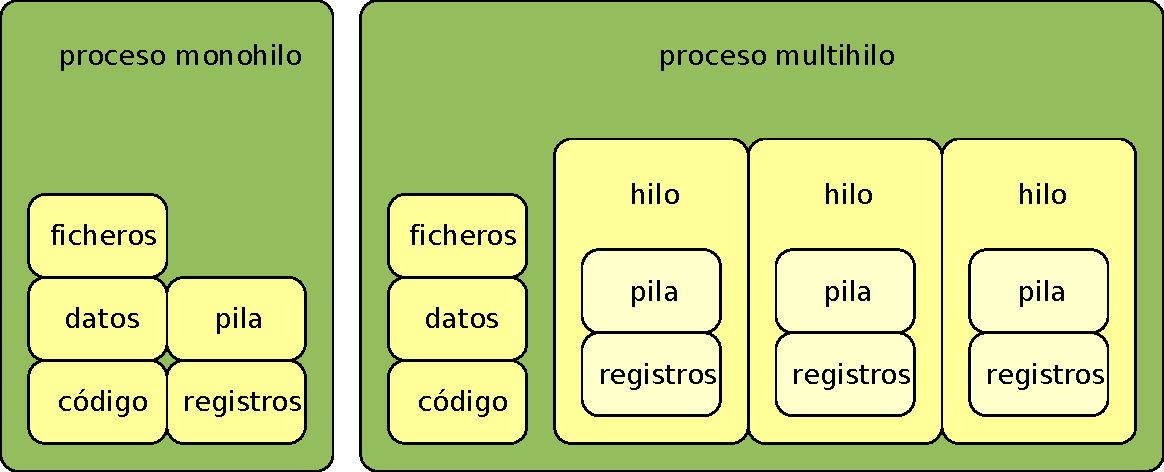
\includegraphics[width=0.8\textwidth]{media/C12_hilos/procesos_multihilo.pdf}
\caption{Esquema comparativo entre procesos monohilo y proceso
multihilo.}\label{fig-multihilo}
\end{figure}

Cada hilo tiene una serie de recursos propios dentro del proceso (véase
la \hyperref[fig-multihilo]{Esquema comparativo entre procesos monohilo
y proceso multihilo.}):

\begin{itemize}
\item
  \textbf{El identificador del hilo} es único para cada hilo y sirve
  para identificarlos, de la misma manera que lo hace el identificador
  de proceso con cada proceso.
\item
  \textbf{El contador de programa} es el registro de la CPU que indica
  la dirección de la próxima instrucción del hilo que debe ser ejecutada
  por la CPU.
\item
  \textbf{Los registros de la CPU}, cuyos valores son diferentes en cada
  hilo, puesto que, aunque todos los hilos ejecutan el mismo programa,
  pueden ejecutar diferentes partes del mismo.
\item
  \textbf{La pila} contiene datos temporales como argumentos y
  direcciones de retorno de las funciones y variables locales. Al igual
  que ocurre con los registros de la CPU, cada hilo necesita su pila
  porque recorre el programa de manera diferente.
\end{itemize}

Sin embargo hay otros recursos que se asignan al proceso, por lo que se
comparten entre todos los hilos del mismo (véase la
\hyperref[fig-multihilo]{Esquema comparativo entre procesos monohilo y
proceso multihilo.}):

\begin{itemize}
\item
  \textbf{El código del programa}. El programa es el mismo para todos
  los hilos.
\item
  \textbf{Los segmentos BSS y de datos y el montón}. Las secciones de
  datos diferentes de la pila son accesibles a todos los hilos. Eso
  quiere decir, por ejemplo, que cualquier hilo puede acceder y
  modificar una variable global o una asignada dinámicamente mediante
  \{clang\_malloc\} o \{cpp\_new\}.
\item
  \textbf{Otros recursos del proceso} como archivos, \emph{sockets},
  tuberías y dispositivos abiertos, regiones de memoria compartida,
  señales, directorio actual de trabajo, entre muchos otros recursos.
\end{itemize}

Esto significa que cada instante, en cada CPU del sistema se puede estar
ejecutando un hilo, del mismo o de distintos procesos en el sistema;
pero la memoria, los archivos y otros recursos pertenecen al proceso del
que cada uno forma parte. Si un hilo reserva memoria o abre un archivo o
un dispositivo y no lo libera antes de terminar, el recurso permanecerá
reservado, no siendo liberado hasta que lo haga otro hilo o el proceso
completo termine. Si un hilo ejecuta una instrucción privilegiada o
intenta acceder a una zona de memoria para la que no tiene permiso, la
condición de error se propaga a todo el proceso. Por tanto, por lo
general, el sistema operativo detendrá el proceso completo del que
formaba parte.

Si se quiere ejecutar varias tareas al mismo tiempo de forma que la
fiabilidad sea máxima, haciendo que los errores en unas no puedan
afectar a las otras, tendremos que olvidarnos de los hilos. Debemos
utilizar diferentes procesos para cada tarea. Así cada tarea tiene sus
propios recursos y su propio espacio de direcciones virtual, lo que
aísla a unas tareas de las otras.

\begin{figure}
\centering
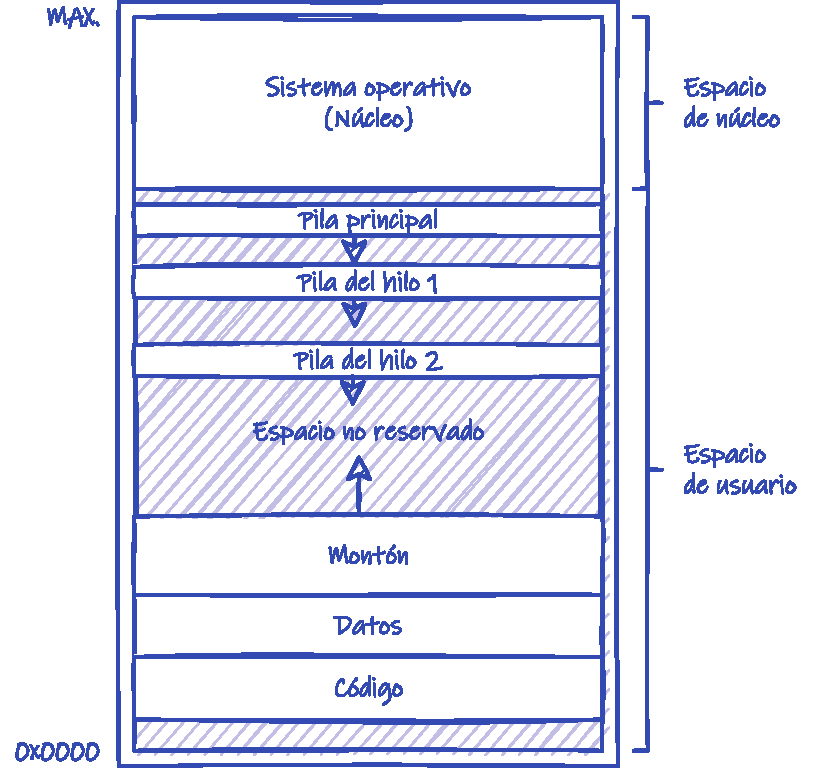
\includegraphics[width=0.8\textwidth]{media/C12_hilos/proceso_multihilo_en_memoria.pdf}
\caption{Anatomía de un proceso multihilo en
memoria.}\label{fig-proceso-multihilo-en-memoria}
\end{figure}

En la \hyperref[fig-proceso-multihilo-en-memoria]{Anatomía de un proceso
multihilo en memoria.} se puede observar como cambia la disposición de
los elementos de un proceso en la memoria cuando es multihilo, respecto
a lo que vimos en el \hyperref[_el_proceso]{???}.

\section{Beneficios}\label{_beneficios}

Son muchos los beneficios que aporta la programación multihilo,
derivados de que ofrece una forma sencilla de que un único proceso pueda
realizar varias tareas al mismo tiempo.

\subsection{Tiempo de respuesta}\label{_tiempo_de_respuesta}

Una aplicación multihilo interactiva puede continuar ejecutando tareas
aunque uno o varios hilos de la misma estén bloqueados o realizando
operaciones muy lentamente, mejorando así el tiempo de respuesta al
usuario.

Por ejemplo, un navegador web multihilo puede gestionar la interacción
del usuario a través de un hilo, mientras el contenido solicitado se
descarga en otro. Para hacer lo mismo en un navegador monohilo habría
que utilizar comunicaciones asíncronas, de lo contrario, mientras el
proceso está en estado \textbf{esperando}, a la espera de que lleguen
los datos a través de la red, no puede atender las acciones del usuario.

El uso de comunicaciones asíncronas para obtener el mismo beneficio
tiene menor coste que usar hilos, pero son más difíciles de programar.

\subsection{Compartición de
recursos}\label{_comparticiuxf3n_de_recursos}

Los hilos no son la única forma de conseguir que un programa realice
varias tareas al mismo tiempo. Una alternativa es que un mismo programa
cree varios procesos hijo, que se comuniquen y coordinen entre sí, para
hacer distintas tareas.

Sin embargo, aunque la programación multiproceso ofrece beneficios
similares a la multihilo, en esta última la comunicación es mucho más
sencilla porque los hilos comparten automáticamente los recursos del
proceso al que pertenecen. De hecho, los hilos no solo comparten la
memoria, sino también otros muchos recursos del proceso, como los
archivos y los dispositivos abiertos. Por lo que los hilos son una forma
más conveniente de ejecutar múltiples tareas al mismo tiempo, que la
programación multiproceso.

Como contrapartida, la programación multiproceso es más fiable, ya que
los errores en un proceso no afectan al resto. Es decir, si un proceso
hijo termina de forma inesperada, el proceso padre puede continuar
ejecutándose sin problemas e incluso crear un nuevo proceso hijo para
sustituir al que ha terminado.

\subsection{Economía}\label{_economuxeda}

Reservar memoria y otros recursos para la creación de un proceso es muy
costoso. Por eso los sistemas operativos modernos han desarrollado
diversas técnicas para que sea lo más eficaz posible.

Aun así, puesto que los hilos comparten los recursos de los procesos a
los que pertenecen, son mucho más económicos de crear. También es más
económico el cambio de contexto entre ellos, ya que hay que guardar y
recuperar menos información a conmutar la ejecución en la CPU entre dos
hilos de un mismo proceso, que entre dos procesos diferentes.

Por ejemplo, en Microsoft Windows crear un proceso puede ser 300 veces
más costoso que un hilo. Mientras que en sistemas Linux es 3 veces más
lento, por la eficiencia de \{linux\_fork\}.

\subsection{Aprovechamiento de las arquitecturas
multiprocesador}\label{_aprovechamiento_de_las_arquitecturas_multiprocesador}

En los sistemas multiprocesador diferentes hilos pueden ejecutarse en
paralelo en distintos procesadores. Por el contrario, un proceso
monohilo solo se puede ejecutar en una CPU a la vez, independientemente
de cuantas CPU estén disponibles para ejecutarlo.

Nuevamente, en los sistemas monohilo se pueden utilizar varios procesos
para aprovechar las arquitecturas multiprocesador. Sin embargo, como
hemos comentado anteriormente, los hilos son más fáciles de programar y
más económicos de crear y gestionar que los procesos.

\subsection{Comparación con soluciones
alternativas}\label{_comparaciuxf3n_con_soluciones_alternativas}

A modo de resumen, los hilos son una forma sencilla de que un único
proceso pueda realizar varias tareas al mismo tiempo, pero no son la
única:

\begin{itemize}
\item
  El uso de \textbf{comunicaciones asíncronas} permite realizar varias
  tareas de E/S al mismo tiempo, sin necesidad de hilos. Suele ser una
  opción más económica que usar hilos, pero también es más difícil de
  programar.
\item
  El uso de \textbf{múltiples procesos} permite realizar varias tareas
  al mismo tiempo, tanto de E/S como de cálculo, y de forma más fiable
  que los hilos. Sin embargo, los procesos suelen ser más caros de crear
  y gestionar que los hilos y no comparten los recursos de forma
  automática, por lo que la comunicación entre ellos es algo más
  complicada.
\end{itemize}

\section{Soporte multihilo}\label{_soporte_multihilo}

Las \textbf{librerías de hilos}{} proporcionan al programador la
interfaz de programación para crear y gestionar los hilos de un proceso.
Por lo general, mediante lenguaje C se puede acceder directamente a la
\textbf{librería de hilos} del sistema. Otros lenguajes proporcionan un
\textbf{librería de hilos} dentro de su \textbf{librería estandar}, que
a su vez se apoya en la \textbf{librería de hilos} del sistema
operativo.

El soporte de hilos en un sistema operativo se puede proporcionar a
\textbf{nivel de usuario} o a \textbf{nivel de núcleo}.

\subsection{Hilos a nivel de usuario}\label{_hilos_a_nivel_de_usuario}

{} El soporte de \textbf{hilos a nivel de usuario} se implementan
mediante un \textbf{librería de hilos} en el espacio de usuario, junto
al código del programa y los datos del proceso, sin requerir ningún
soporte especial por parte del núcleo del sistema operativo. Por tanto,
como se puede observar en el lado derecho de la
\hyperref[fig-comparaciuxf3n-soporte-de-hilos]{Comparación de hilos a
nivel de usuario y a nivel de núcleo.}, estos hilos existen desde el
punto de vista del proceso y del programa que ejecuta, pero no para el
sistema operativo. El planificador de la CPU asigna tiempo de CPU a los
procesos, mientras que la \textbf{librería de hilos} de cada proceso
reparte el tiempo de ejecución del proceso entre los diferentes hilos de
este.

\begin{figure}
\centering
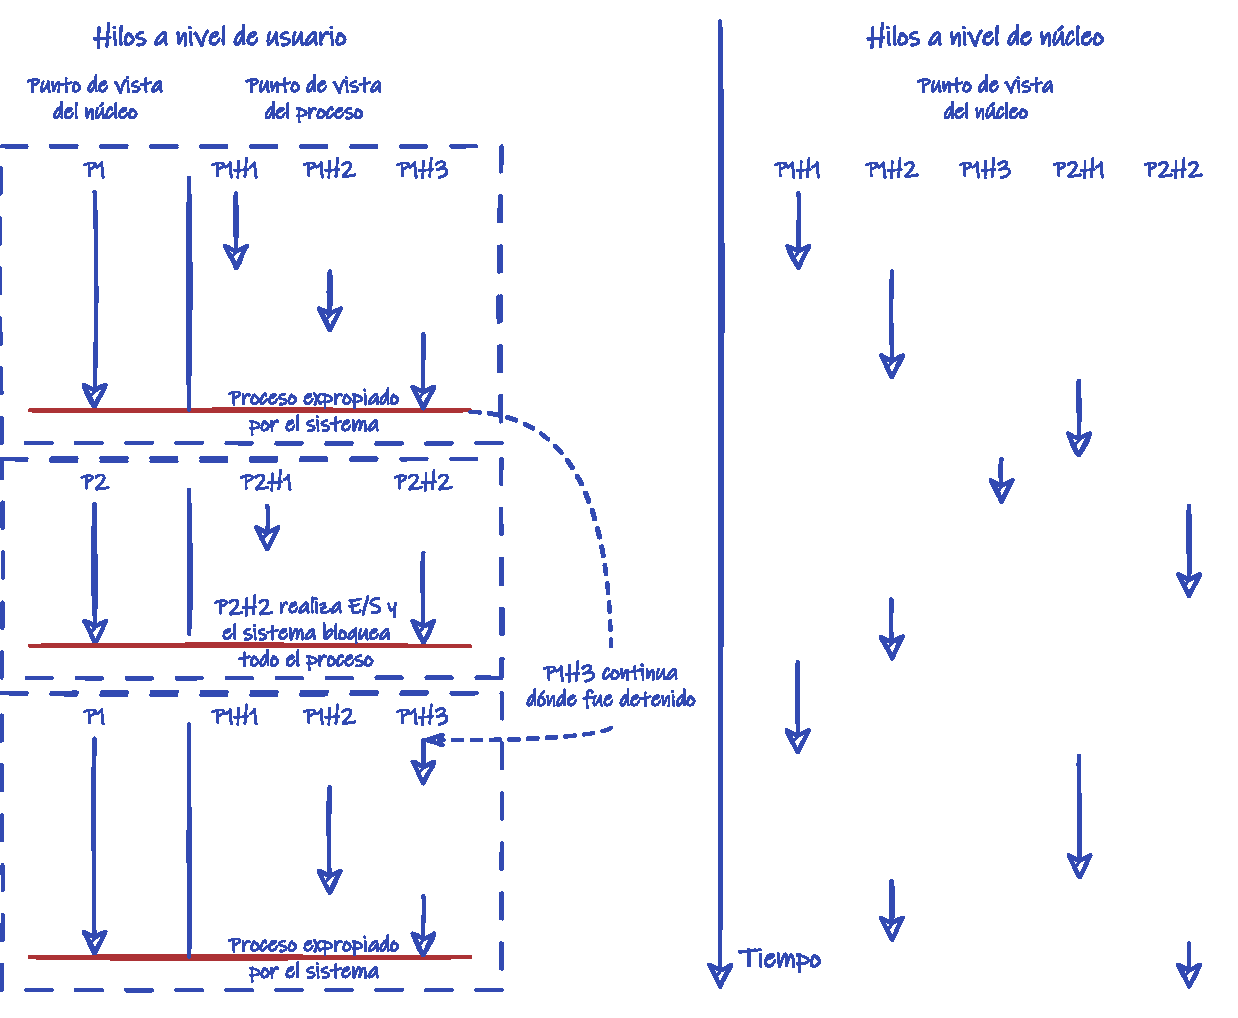
\includegraphics[width=0.8\textwidth]{media/C12_hilos/comparación_soporte_de_hilos.pdf}
\caption{Comparación de hilos a nivel de usuario y a nivel de
núcleo.}\label{fig-comparaciuxf3n-soporte-de-hilos}
\end{figure}

Como el código y los datos de la librería residen en el espacio de
usuario, invocar una función de la misma se reduce a una simple llamada
a una función, evitando el coste de hacer llamadas al sistema.

\subsection{Hilos a nivel de núcleo}\label{_hilos_a_nivel_de_nuxfacleo}

{} Se habla de \textbf{hilos a nivel de núcleo}, cuando el núcleo del
sistema es el encargado de ofrecer el soporte multihilo. El código y los
datos de la \textbf{librería de hilos}, mediante la cual los
programadores pueden solicitar la creación y gestión de los hilos,
reside en el espacio del núcleo. Por tanto, para invocar una función de
la \textbf{librería de hilos} es necesario hacer una llamada al sistema.
Obviamente, la librería del sistema ofrece las funciones necesarias para
realizar estas llamadas al sistema de forma sencilla.

La implementación del soporte de hilos en el núcleo implica cambios
respecto a lo que hemos visto hasta el momento de la gestión de
procesos, puesto que, en estos sistemas, es el hilo la unidad básica de
uso de la CPU, como se ilustra en la
\hyperref[fig-comparaciuxf3n-soporte-de-hilos]{Comparación de hilos a
nivel de usuario y a nivel de núcleo.}. Es decir, son los hilos los que
se mueven por los estados del
\hyperref[fig-diagrama-estado-proceso]{???} y las colas de la
\hyperref[fig-colas-de-planificaciuxf3n-procesos]{???}, en lugar de los
procesos. En estos sistemas, el planificador de la CPU selecciona un
hilo para ejecutarse en la CPU de entre todos los que están en el estado
\textbf{preparado} en el sistema y el \textbf{cambio de contexto} asigna
la CPU a un hilo distinto al que la tiene asignada en el momento actual,
que puede ser del mismo o de diferente proceso.

Aparte del \textbf{PCB} que vimos en el
\hyperref[_bloque_de_control_de_proceso]{???}, ahora el sistema
operativo también gestiona una estructura llamada \textbf{bloque de
control del hilo}{} o {}TCB (\emph{Thread Control Block}) para cada hilo
en el sistema, donde se guarda información sobre su estado de actividad
actual. Por tanto, es en \textbf{TCB} ---y no en el \textbf{PCB}---
donde se guarda la información privada del hilo necesaria para la
gestión de los estados y para el cambio de contexto, como: los valores
de los registros de la CPU y el contador de programa, el estado o la
información de planificación de la CPU; además de un puntero al
\textbf{PCB} al que pertenece el hilo con el resto de la información
privada del proceso.

\subsection{Implementaciones}\label{_implementaciones}

En la actualidad, en los diferentes sistemas operativos se pueden
encontrar librerías de ambos tipos.

Por ejemplo, la librería de hilos de Windows API se implementa en el
núcleo\hyperref[Win32-UsingProcessesAndThreads]{???} mientras que la
librería de hilos \{pthreads\} ---frecuentemente utilizada en los
sistemas POSIX--- puede ser de ambos tipos, dependiendo solamente del
sistema donde se implemente. En Linux y en la mayor parte de los UNIX
modernos, POSIX Threads se implementa en el núcleo del sistema.

\section{Modelos multihilo}\label{_modelos_multihilo}

En base a lo anterior, sabemos que hay sistemas que implementan
\textbf{hilos a nivel de núcleo} mientras otros los hacen a
\textbf{nivel de usuario}. Sin embargo, también existen sistemas donde
se combinan ambos.

Para comparar las diferentes opciones que tienen los diseñadores de un
sistema en cuanto al soporte de hilos, se definen los \textbf{modelos
multihilo} en base a la relación entre \textbf{hilos de usuario} e
\textbf{hilos de núcleo}. Aquí entendemos por \textbf{hilos de núcleo} a
estas secuencias de instrucciones tal y como las ve el programa en el
espacio de usuario. Mientras que el concepto de \textbf{hilos de núcleo}
corresponde con como las ve el núcleo del sistema.

\subsection{Muchos a uno (N:1)}\label{_muchos_a_uno_n1}

{} {} En el modelo \textbf{muchos a uno} muchos \textbf{hilos de
usuario} son mapeados en \textbf{un único hilo de núcleo}. El
planificador de la CPU en el núcleo reparte el tiempo de CPU entre los
diferentes \textbf{hilos de núcleo} en el sistema, mientras que la
\textbf{librería de hilos} en cada proceso reparte el tiempo de
ejecución del \textbf{hilo de núcleo} del proceso entre múltiples
\textbf{hilos de usuario} (véase la
\hyperref[fig-modelo-muchos-a-uno]{Modelo muchos a uno (N:1).}).

\begin{figure}
\centering
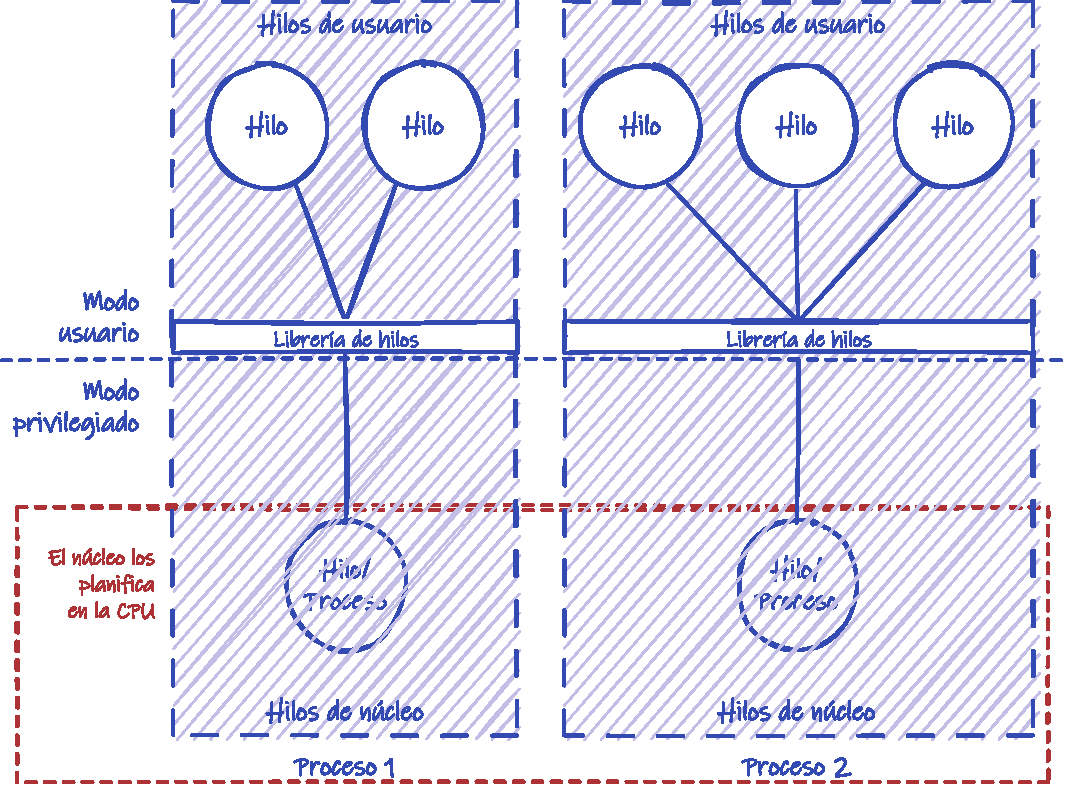
\includegraphics[width=0.8\textwidth]{media/C12_hilos/modelo_muchos_a_uno.pdf}
\caption{Modelo muchos a uno (N:1).}\label{fig-modelo-muchos-a-uno}
\end{figure}

Los sistemas modernos son multihilo, por lo que al crearse un proceso
siempre se crea con un \textbf{hilo de núcleo} inicial, que es al que el
núcleo asigna tiempo de CPU. Sin embargo, los sistemas más antiguos no
tienen ningún soporte de hilos en el núcleo, por lo que no hay
\textbf{hilos de núcleo}. En este sentido, quizás sería más correcto
definir el modelo \textbf{muchos a uno} como aquel en el que muchos
\textbf{hilos de usuario} son mapeados en una «única entidad
planificable en la CPU». En los sistemas más antiguos estas entidades
son los procesos, de forma que, bajo este \textbf{modelo multihilo} los
\textbf{hilos de usuario} realmente se reparten el tiempo de ejecución
del proceso al que pertenecen.

El modelo \textbf{muchos a uno} corresponde al caso en el que solo se
implementan \textbf{hilos a nivel de usuario}, que es el caso ilustrado
a la izquierda en la
\hyperref[fig-comparaciuxf3n-soporte-de-hilos]{Comparación de hilos a
nivel de usuario y a nivel de núcleo.}.

\subsubsection{Ventajas e
inconvenientes}\label{_ventajas_e_inconvenientes}

La principal \textbf{ventaja} de este modelo es su bajo coste, por lo
que resulta ideal cuando la cantidad de hilos a crear ---el nivel de
concurrencia--- va a ser muy alta:

\begin{itemize}
\item
  Los \textbf{hilos de usuario} son muy baratos de crear porque la
  gestión de hilos se hace con una librería en el espacio de usuario,
  dentro del proceso. Mientras que los \textbf{hilos de núcleo} pueden
  necesitar más recursos del sistema, como espacio en la tabla de hilos
  del sistema y en otras estructuras de gestión.
\item
  La invocación de las funciones de la \textbf{librería de hilos} se
  hace por medio de simples llamadas a funciones, que son menos costosas
  que las llamadas al sistema necesarias cuando el soporte de hilos se
  implementa en el núcleo.
\item
  Se necesitan menos cambios de contexto. Los cambios de contexto, que
  ocurren cuando se transfiere el control de la CPU, pueden ser
  operaciones costosas. En el modelo \textbf{muchos a uno} pueden
  ocurrir cambios de contexto en el núcleo al intercambiar procesos en
  la CPU, pero el intercambio de hilos se gestiona en el propio proceso,
  lo que suele ser más rápido que hacerlo en el núcleo.
\end{itemize}

Mientras que estos son algunos posibles \textbf{inconvenientes}:

\begin{itemize}
\item
  Los hilos de un mismo proceso no se pueden ejecutar en paralelo en
  sistemas multiprocesador, por lo que este modelo no permite aprovechar
  ese tipo de sistemas. El motivo es que la librería de hilos en espacio
  de usuario no tiene acceso a los procesadores del sistema. Solo conoce
  el proceso en el que se ejecuta y reparte el tiempo de ejecución del
  proceso entre los distintos hilos.

  El núcleo del sistema si ve los diferentes procesadores, pero
  desconoce la existencia de los hilos dentro de los procesos. Solo ve
  procesos que deben ejecutarse en las distintas CPU.
\item
  Un hilo puede bloquear la ejecución del resto de los hilos de su
  proceso, en determinadas circunstancias.

  Si uno de los hilos solicita al sistema operativo una operación que
  deba ser bloqueada a la espera ---por ejemplo,operaciones de E/S sobre
  archivos, comunicaciones o esperar a que otro proceso termine--- todo
  el proceso es puesto como \emph{esperando} por el sistema operativo,
  no pudiendo ejecutarse otros hilos del mismo proceso en la CPU,
  mientras tanto. Para evitar en parte este problema, es frecuente que
  las implementaciones de este modelo ofrezcan versiones especiales de
  estas operaciones, con capacidad para evitar el bloqueo total del
  proceso, en función de si el sistema operativo tiene el soporte
  adecuado para ello.
\end{itemize}

Por tanto, este modelo no es una opción si lo que interesa es aprovechar
el paralelismo en sistemas multiprocesador, para intentar realizar
ciertas operaciones en menos tiempo.

\subsubsection{Operaciones bloqueantes}\label{_operaciones_bloqueantes}

El problema del bloqueo de procesos ocasionado por operaciones de E/S
que pongan al proceso en estado \emph{esperando} puede ser evitado
interceptando las llamadas a funciones de la librería del sistema, para
evitar el uso de llamadas al sistema que se puedan bloquear y
sustituirlas por versiones equivalentes pero asíncronas.

Obviamente, la \textbf{librería de hilos} intercambia el \textbf{hilo de
usuario} en ejecución cuando el que se está ejecutando finaliza. Además,
generalmente, tiene funciones para que el \textbf{hilo de usuario} en
ejecución se duerma ---\texttt{sleep()}--- o para que espere a que otro
hilo termine ---\texttt{wait()} o \texttt{join()}. En ambos casos, el
\textbf{hilo de usuario} queda bloqueado y la \textbf{librería de hilos}
asigna otro hilo al \textbf{hilo de núcleo} para su ejecución.

Por ejemplo, en la
\hyperref[fig-modelo-a-uno-operaciuxf3n-bloqueante]{Diagrama de
secuencia del bloqueo del proceso en el modelo muchos a uno.} se ilustra
como el \emph{Hilo 1} llama a la función \texttt{yield()} de la
\textbf{librería de hilos}, provocando su intercambio con el \emph{Hilo
2}. La función \texttt{yield()} suele estar presente en algunas
\textbf{librerías de hilos}, con el objeto de que los hilos puedan
indicar puntos del programa en los que quieren dejar tiempo de ejecución
para otros hilos, de forma voluntaria.

\begin{figure}
\centering
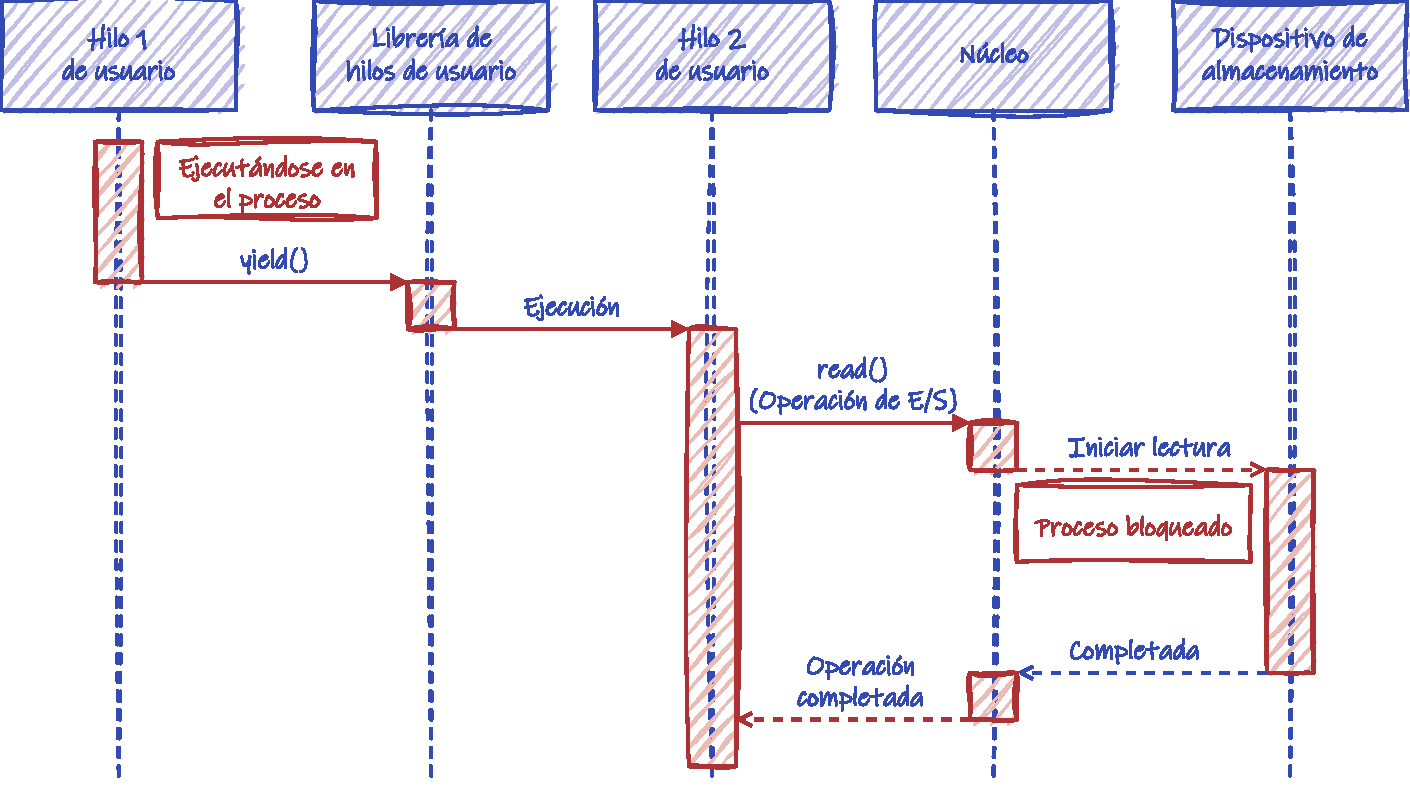
\includegraphics[width=0.8\textwidth]{media/C12_hilos/muchos_a_uno_operación_bloqueante.pdf}
\caption{Diagrama de secuencia del bloqueo del proceso en el modelo
muchos a uno.}\label{fig-modelo-a-uno-operaciuxf3n-bloqueante}
\end{figure}

Sin embargo, en la
\hyperref[fig-modelo-a-uno-operaciuxf3n-bloqueante]{Diagrama de
secuencia del bloqueo del proceso en el modelo muchos a uno.} también
vemos que \emph{Hilo 2} invoca la llamada al sistema \texttt{read()}
para leer un archivo. Desde el punto de vista del núcleo, esa llamada la
realiza el proceso, por lo que es bloqueado, hasta que la operación de
lectura del archivo se completa. Al proceso nunca se le asignará la CPU
mientras esté en estado \emph{esperando}, por lo que ni \emph{Hilo 1} ni
ningún otro \textbf{hilo de usuario} del proceso podrá ejecutarse.

La solución, como hemos comentado, es que la \textbf{librería de hilos}
proporcione sus propias versiones de las llamadas al sistema que pueden
poner al proceso en estado \emph{esperando}. Por ejemplo, en la
\hyperref[fig-modelo-a-uno-operaciuxf3n-bloqueante]{Diagrama de
secuencia del bloqueo del proceso en el modelo muchos a uno.} el
\emph{Hilo 2} no usa la llamada al sistema \texttt{read()} sino una
función \texttt{read()} proporcionada por la \textbf{librería de hilos}.

Para implementar su \texttt{read()}, la \textbf{librería de hilos} usa
una versión asíncrona de la llamada al sistema. Es decir, una versión
donde se le indica al sistema que se quiere hacer una operación de E/S,
pero el proceso no entra en estado de espera mientras ocurre. En su
lugar, el proceso retorna inmediatamente de la llamada al sistema y
sigue ejecutándose en la CPU, lo que permite que la \textbf{librería de
hilos} comience a ejecutar \emph{Hilo 1} en el lugar de \emph{Hilo 2}.
Es decir, desde el punto de vista de \emph{Hilo 2}, la función
\texttt{read()} de la \textbf{librería de hilos} es bloqueante.

\begin{figure}
\centering
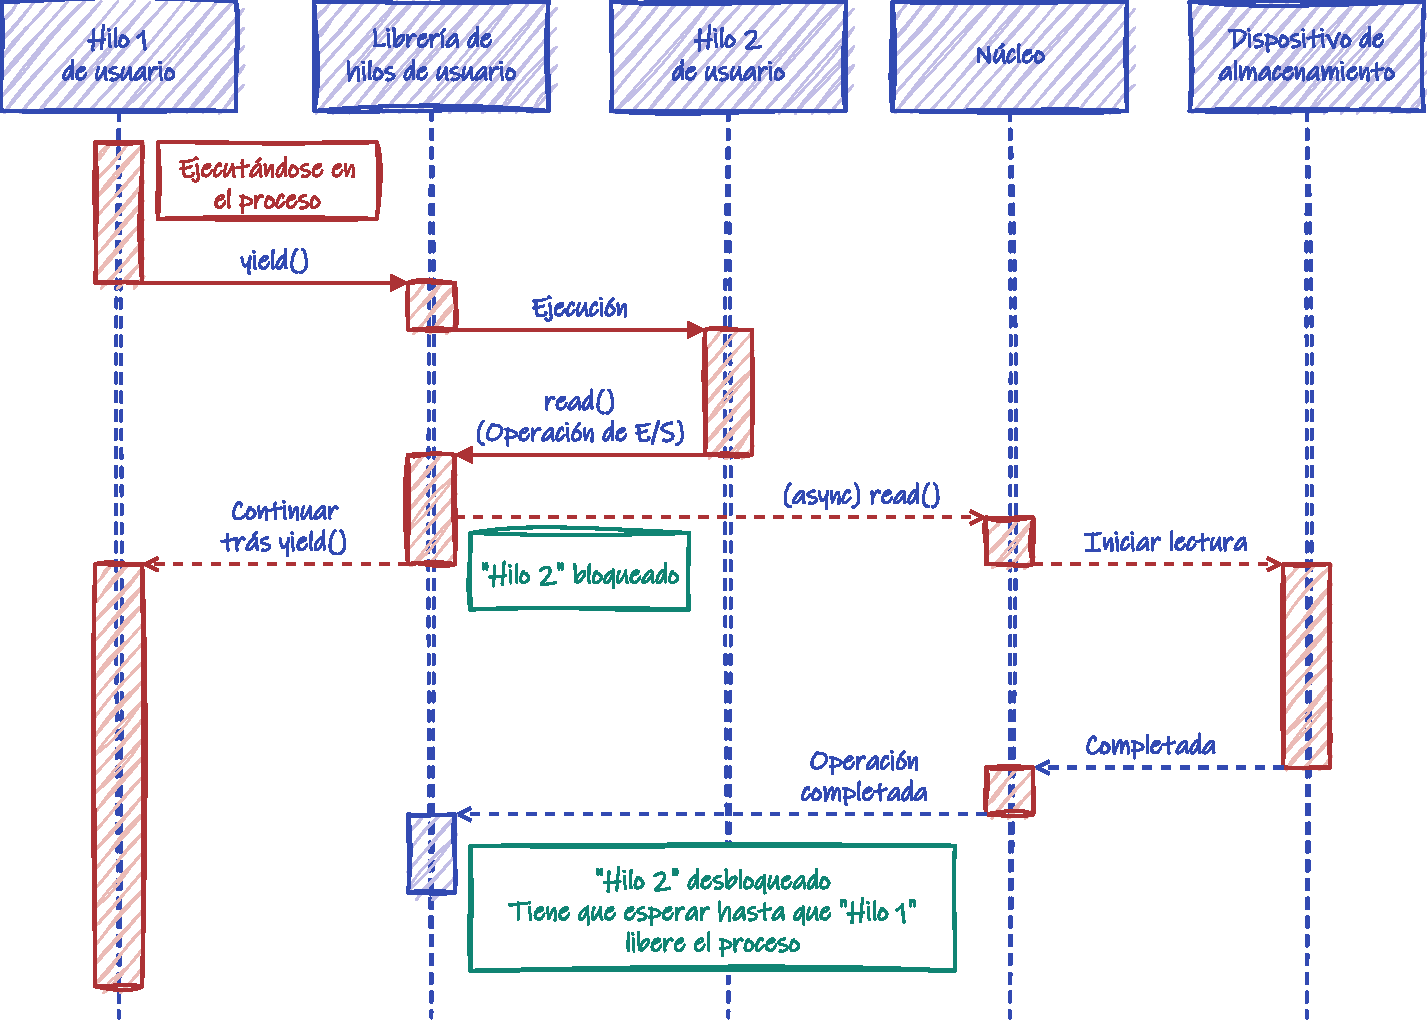
\includegraphics[width=0.8\textwidth]{media/C12_hilos/muchos_a_uno_operación_async.pdf}
\caption{Diagrama de secuencia de la solución al bloqueo del proceso en
el modelo muchos a uno.}\label{fig-modelo-a-uno-operaciuxf3n-async}
\end{figure}

Más adelante, el sistema operativo notificará a la \textbf{librería de
hilos} que la operación ha sido realizada, por lo que los datos ya están
disponibles en la memoria para ser usados. En ese momento, \emph{Hilo 2}
vuelve al estado \emph{preparado} para volver a ser planificado por la
\textbf{librería de hilos} cuando sea posible.

Este procedimiento es complejo y requiere versiones no bloqueantes de
todas las llamadas al sistema, lo que puede que no siempre se cumpla.
Por lo general, cualquier sistema operativo moderno ofrece versiones
asíncronas de todas las operaciones de E/S, pero puede haber otras
llamadas al sistema que puedan poner al proceso en estado
\emph{esperando} y que no tengan versión asíncrona.

\subsubsection{Implementaciones}\label{_implementaciones_2}

A este modelo de hilos también se lo denomina
\href{https://en.wikipedia.org/wiki/Green_threads}{Green Threads}. En
Java 1.1 era el único modelo soportado ---ya que los hilos se
implementaban en la máquina virtual de Java, independientemente del
soporte del sistema operativo--- pero debido a sus limitaciones se
implementó el soporte de hilos nativos del sistema operativo.

Otras implementaciones de este modelo son las
\href{https://docs.microsoft.com/en-us/windows/win32/procthread/fibers}{fibras}
y
\href{https://docs.microsoft.com/en-us/windows/win32/procthread/user-mode-scheduling}{UMS}
de Windows API, \{stackless\_python\} y
\href{http://www.gnu.org/software/pth/}{GNU Portable Threads}.

\subsection{Uno a uno (1:1)}\label{_uno_a_uno_11}

{} {} En el modelo \textbf{muchos a uno} un \textbf{hilo de usuario} se
mapea en \textbf{un único hilo de núcleo}.

Por lo general, este modelo corresponde al caso de los sistemas que solo
soportan \textbf{hilos a nivel de núcleo}. En este caso, la
\textbf{librería de hilos} se implementa en el núcleo, por lo que las
entidades que planifica el núcleo en la CPU son los \textbf{hilos de
núcleo} y los procesos pueden gestionar estos hilos mediante llamadas al
sistema (véase la \hyperref[fig-modelo-uno-a-uno]{Modelo uno a uno
(1:1).}).

\begin{figure}
\centering
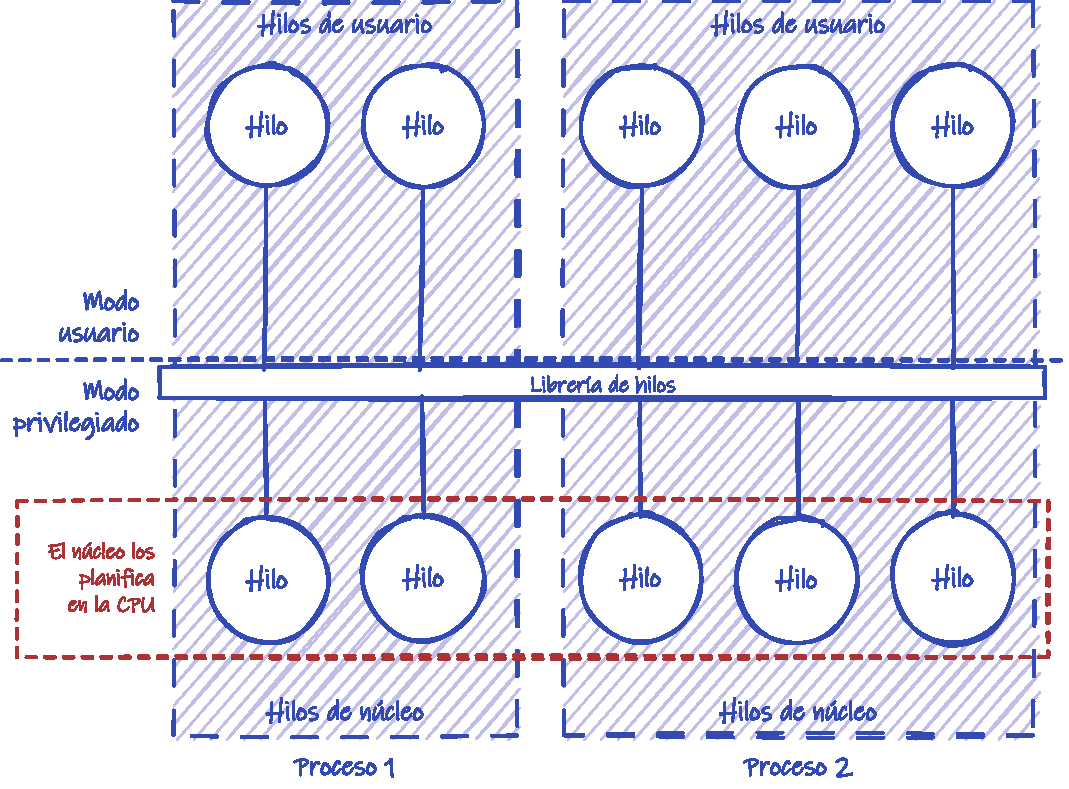
\includegraphics[width=0.8\textwidth]{media/C12_hilos/modelo_uno_a_uno.pdf}
\caption{Modelo uno a uno (1:1).}\label{fig-modelo-uno-a-uno}
\end{figure}

Es importante tener en cuenta que, a efectos prácticos, los
\textbf{hilos de usuario} de la \hyperref[fig-modelo-uno-a-uno]{Modelo
uno a uno (1:1).} no son hilos diferentes a los \textbf{hilos de
núcleo}. Realmente, son los mismos \textbf{hilos de núcleo}, pero vistos
desde la perspectiva del programa en el modo usuario, como se ilustra a
la derecha en la
\hyperref[fig-comparaciuxf3n-soporte-de-hilos]{Comparación de hilos a
nivel de usuario y a nivel de núcleo.}.

\subsubsection{Ventajas e
inconvenientes}\label{_ventajas_e_inconvenientes_2}

Las principales \textbf{ventajas} de este modelo son:

\begin{itemize}
\item
  Permite a otros hilos del mismo proceso ejecutarse aun cuando uno de
  ellos haga una llamada al sistema que debe bloquearse. El núcleo se
  encarga de ponerlo en espera y planificar en la CPU a otro de los
  hilos preparados para ejecutarse de entre todos los existentes en el
  sistema.
\item
  Permite paralelismo en sistemas multiprocesador, ya que diferentes
  hilos pueden ser planificados por el núcleo en distintos procesadores.
\end{itemize}

Mientras que estos son algunos posibles \textbf{inconvenientes}:

\begin{itemize}
\item
  Crear hilos puede tener mayor coste. En este caso, crear un hilo para
  un proceso implica crear y gestionar ciertas estructuras de datos en
  el núcleo. Debido a que la cantidad de memoria disponible para el
  núcleo suele estar limitada, muchos sistemas restringen la cantidad
  máxima de \textbf{hilos de núcleo} soportados.
\item
  La gestión de los hilos se hace con una librería en el espacio de
  núcleo, lo que requiere que el proceso haga llamadas al sistema para
  gestionarlos. Esto suele tener mayor coste que invocar simplemente una
  función, como ocurre en el modelo \textbf{muchos a uno}.
\end{itemize}

\subsubsection{Implementaciones}\label{_implementaciones_3}

El modelo \textbf{uno a uno} se utiliza en la mayor parte de los
sistemas operativos multihilo modernos. Linux, Microsoft Windows
---desde Windows 95--- \{solaris\} 9 y superiores, macOS y la familia de
UNIX BSD; son ejemplos de sistemas operativos que utilizan el modelo
\textbf{uno a uno}.

\subsection{Muchos a muchos (M:N)}\label{_muchos_a_muchos_mn}

{} {} En teoría debería ser posible aprovechar lo mejor de los dos
modelos anteriores con una \textbf{librería de hilos} en el núcleo, para
crear \textbf{hilos de núcleo}, y otra en el espacio de usuario, para
crear \textbf{hilos de usuario}. Así los desarrolladores pueden utilizar
la \textbf{librería de hilos} en el espacio de usuario para crear tantos
hilos como quieran y que estos se ejecuten sobre los \textbf{hilos de
núcleo} de su proceso.

El planificador de la \textbf{librería de hilos} en espacio de usuario
se encarga de determinar como se reparte el tiempo de ejecución de cada
\textbf{hilo de núcleo} entre los \textbf{hilos de usuario}. Mientras
que el planificador de la CPU asigna la CPU a alguno de los
\textbf{hilos de núcleo} del sistema (véase la
\hyperref[fig-modelo-muchos-a-muchos]{Modelo muchos a muchos (M:N).}).

\begin{figure}
\centering
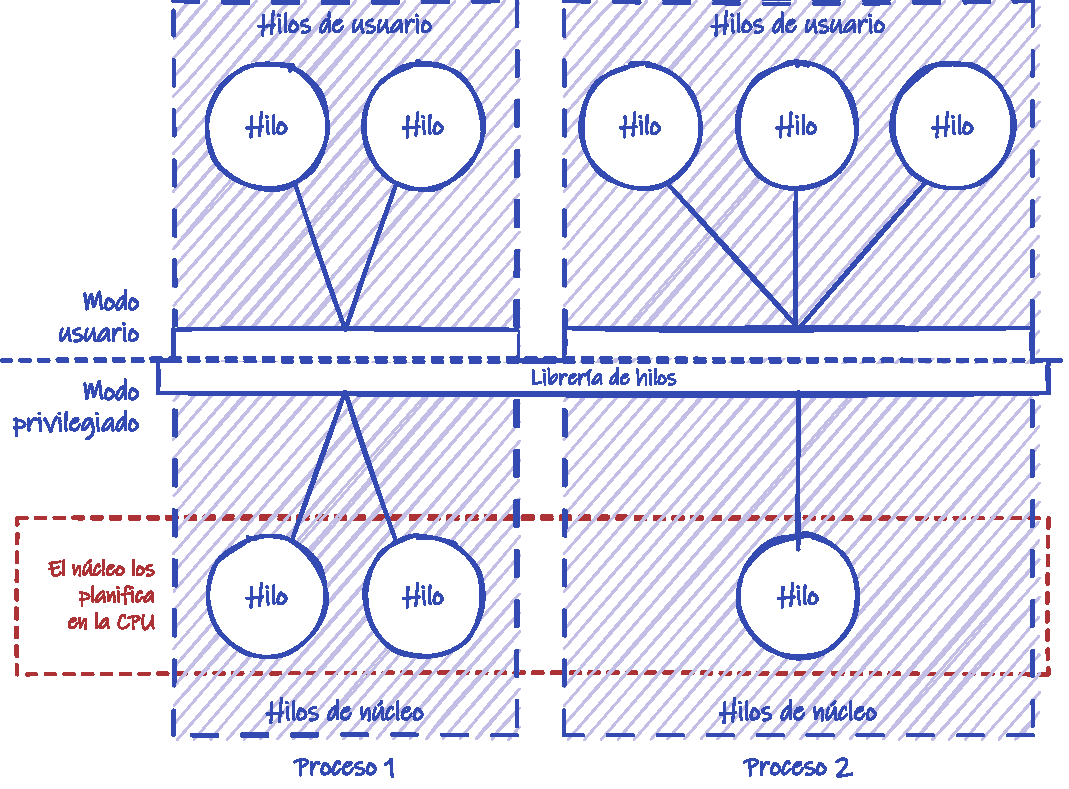
\includegraphics[width=0.8\textwidth]{media/C12_hilos/modelo_muchos_a_muchos.pdf}
\caption{Modelo muchos a muchos
(M:N).}\label{fig-modelo-muchos-a-muchos}
\end{figure}

\subsubsection{Activación del
planificador}\label{_activaciuxf3n_del_planificador}

En el modelo \textbf{muchos a muchos} es conveniente que exista cierto
grado de coordinación entre el núcleo y la \textbf{librería de hilos}
del espacio de usuario. Dicha comunicación tiene como objeto ajustar
dinámicamente el número de \textbf{hilos de núcleo} para garantizar la
máxima eficiencia.

\begin{figure}
\centering
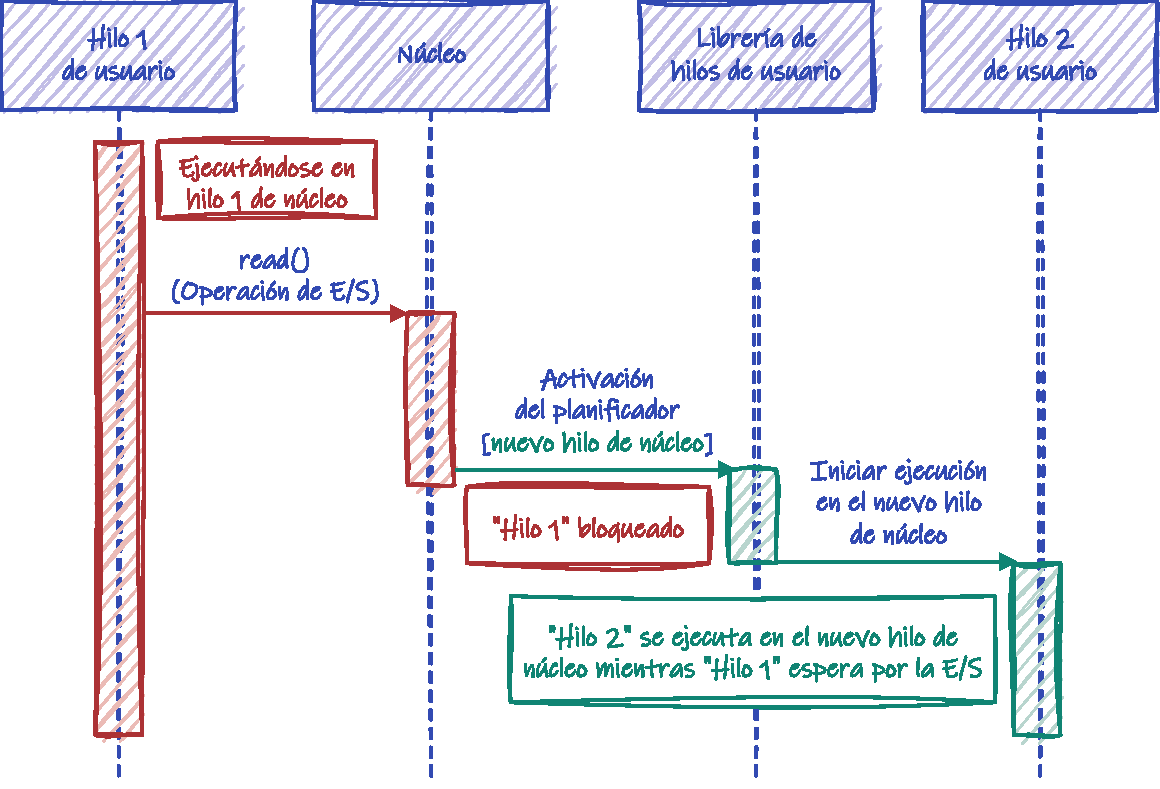
\includegraphics[width=0.8\textwidth]{media/C12_hilos/activación_del_planificador.pdf}
\caption{Diagrama de secuencia del mecanismo de activación del
planificador.}\label{fig-activaciuxf3n-del-planificador}
\end{figure}

Uno de los esquemas de comunicación se denomina \textbf{{}activación del
planificador} y consiste en que el núcleo informa a la \textbf{librería
de hilos} en espacio de usuario que una llamada al sistema, realizada
por uno de sus hilos de usuario, va a bloquear un \textbf{hilo de
núcleo} del proceso cuyos hilos gestiona. Antes de dicha notificación,
el núcleo se encarga de crear un nuevo \textbf{hilo de núcleo} en el
proceso y se lo pasa a la \textbf{librería de hilos} en la notificación
(véase la \hyperref[fig-activaciuxf3n-del-planificador]{Diagrama de
secuencia del mecanismo de activación del planificador.}). Así, el
planificador de la librería puede asignarle alguno de los otros
\textbf{hilos de usuario}, evitando el bloqueo completo del proceso si
no quedan \textbf{hilos de núcleo} disponibles, y ajustando el número de
\textbf{hilos de núcleo} dinámicamente, según las necesidades

\subsubsection{Ventajas e
inconvenientes}\label{_ventajas_e_inconvenientes_3}

Las principales \textbf{ventajas} de este modelo son:

\begin{itemize}
\item
  Permite paralelismo en sistemas multiprocesador, ya que diferentes
  \textbf{hilos de núcleo} pueden ser planificados en distintos
  procesadores y en cada uno puede ejecutarse cualquier \textbf{hilo de
  usuario} de su proceso.
\item
  Permite a otro \textbf{hilo de usuario} del mismo proceso ejecutarse
  cuando un hilo hace una llamada al sistema que debe bloquearse. Si
  esto ocurre el correspondiente hilo de núcleo se queda bloqueado, pero
  el resto de los \textbf{hilos de usuario} pueden seguir ejecutándose
  en los otros \textbf{hilos de núcleo} del proceso (véase el
  \hyperref[_activaciuxf3n_del_planificador]{Activación del
  planificador}).
\end{itemize}

Mientras que el principal \textbf{inconveniente} es su complejidad para
implementarlo y la dificultad de coordinar el planificador de la
librería de hilos en espacio de usuario con el planificador de la CPU
para obtener el mejor rendimiento.

Como veremos en el \hyperref[planificaciuxf3n_de_la_cpu]{???}, los
planificadores de la CPU modernos intentan clasificar los \textbf{hilos
de núcleo} para ordenarlos de la forma más óptima en el acceso a la CPU.
Por ejemplo, no es lo mismo una tarea de cálculo, que necesita usar
intensivamente la CPU, que copia datos de la red o del sistema de
archivos. Generalmente, primero se planifican las segundas, dejando para
el final las tareas intensivas en el uso de la CPU.

En el modelo \textbf{muchos a muchos} un mismo \textbf{hilo de núcleo}
se pueden ejecutar diferentes \textbf{hilos de usuario} que pueden ser
de distinto tipo. Por tanto, cualquier clasificación que haga el
planificador de la CPU puede ser incorrecta en cuanto la
\textbf{librería de hilos} en espacio de usuario cambie el \textbf{hilo
de usuario} que se está ejecutando un \textbf{hilo de núcleo} por otro
diferente. La solución a este problema pasa porque la \textbf{librería
de hilos} en espacio de usuario y el planificador de la CPU intercambien
información sobre sus hilos y se coordinen.

Debido a estas dificultades, muchos sistemas actuales han optado
finalmente por el modelo \textbf{uno a uno}, concentrando esfuerzos en
reducir el coste de creación de \textbf{hilos a nivel de núcleo}, con el
objeto de que haya poca ventaja en implementar también \textbf{hilos a
nivel de usuario}.

Esto no significa que actualmente no se puedan obtener las ventajas del
modelo \textbf{muchos a muchos} en casos en los que puede ser
beneficioso. Para esos casos los desarrolladores pueden utilizar
librerías o lenguajes específicos, con implementaciones diseñadas para
crear un gran número de \textbf{hilos de usuario} con un coste mínimo,
sobre la librería de hilos de los sistemas operativos actuales.

\subsubsection{Implementaciones}\label{_implementaciones_4}

Este modelo se soportaba en sistemas \{freebsd\} y versiones antiguas de
\{netbsd\}, así como en UNIX comerciales, como: \{solaris\} 8 y
anteriores, \{irix\}, \{hpux\} y \{tru64\}. Microsoft Windows también
soportaba este modelo ---a partir de Windows 7 y hasta Windows 10---
gracias a incorporar un mecanismo denominado \emph{planificación en modo
usuario}\hyperref[Win32-UserModeScheduling]{???}.

Algunos lenguajes de programación implementan el modelo \textbf{muchos a
muchos} sobre el modelo \textbf{uno a uno} soportado por la mayoría de
sistemas operativos modernos. Ese es el caso de \{golang\},
\href{https://es.wikipedia.org/wiki/Erlang}{Erlang},
\href{https://es.wikipedia.org/wiki/Elixir_(lenguaje_de_programaci\%C3\%B3n)}{Elixir}
y
\href{https://blogs.oracle.com/javamagazine/post/java-loom-virtual-threads-platform-threads}{Java}.

\subsection{Dos niveles}\label{_dos_niveles}

Existe una variación del modelo \textbf{muchos a muchos} donde, además
de funcionar de la forma comentada anteriormente, se permite que un
\textbf{hilo de usuario} quede ligado indefinidamente a un único
\textbf{hilo de núcleo}, como en el modelo \textbf{uno a uno}.

Esta variación se denomina, en ocasiones, modelo de \textbf{dos niveles}
(véase la \hyperref[fig-modelo-de-dos-niveles]{Modelo de dos niveles.}).

\begin{figure}
\centering
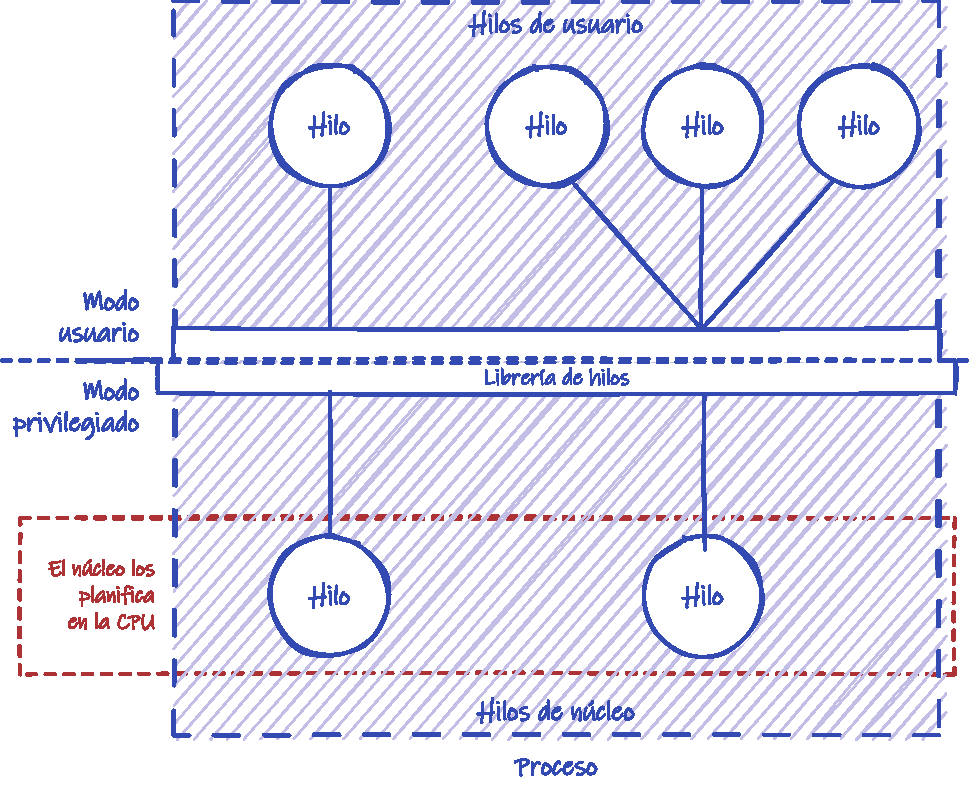
\includegraphics[width=0.8\textwidth]{media/C12_hilos/modelo_de_dos_niveles.pdf}
\caption{Modelo de dos niveles.}\label{fig-modelo-de-dos-niveles}
\end{figure}

\subsubsection{Ventajas e
inconvenientes}\label{_ventajas_e_inconvenientes_4}

El modelo de \textbf{dos niveles} presenta los mismos inconvenientes que
el modelo \textbf{muchos a muchos}, con algunas \textbf{ventajas} en
casos de uso concretos:

\begin{itemize}
\item
  Al vincular un \textbf{hilo de usuario} a un \textbf{hilo de núcleo}
  se asegura la disponibilidad del recurso, lo que puede ser interesante
  si un \textbf{hilo de usuario} es particularmente importante para el
  rendimiento de la aplicación.
\item
  En sistemas con múltiples procesadores o núcleos, puede interesar que
  un \textbf{hilo de usuario} se ejecute siempre en el mismo procesador
  o núcleo para aprovechar la caché y mejorar el rendimiento. Al
  vincular un \textbf{hilo de usuario} a un \textbf{hilo de núcleo} y
  configurar este último para que siempre se planifique en el mismo
  procesador, se está asegurando esta misma condición para el
  \textbf{hilo de usuario} correspondiente.
\end{itemize}

\subsection{El coste de crear hilos y la elección de
modelo}\label{_el_coste_de_crear_hilos_y_la_elecciuxf3n_de_modelo}

Hemos comentado que el modelo \textbf{muchos a uno} debe ser,
teóricamente, «más ligero» que el modelo \textbf{uno a uno}. También
hemos dicho que el modelo \textbf{muchos a muchos}, teóricamente,
permite conservar esa ventaja, al tiempo que ofrece los beneficios del
modelo \textbf{uno a uno}, en lo que respecta al aprovechamiento de los
sistemas multiprocesador. Sin embargo, debemos tener en cuenta que la
diferencia real puede variar en función de múltiples factores.

Un criterio común hasta la década de los 2000, era que el modelo
\textbf{uno a uno} era adecuado hasta varias decenas hilos ---a lo sumo,
en torno a 100 o, quizás, a unos pocos cientos de hilos--- por proceso,
mientras que el modelo \textbf{muchos a uno} podía llegar a varios miles
de hilos.

La principal limitación en la cantidad de \textbf{hilos de usuario} del
modelo \textbf{muchos a uno} estaba en el tamaño del espacio de
direcciones del proceso. Por ejemplo, en las versiones de Windows de 32
bits, los procesos dispone de 2 GiB de su espacio de direcciones para
código y datos. Como cada \emph{fibra} ---que es como se llama a los
hilos del modelo multihilo \textbf{muchos a uno} que implementa la API
Win32 de Windows--- necesita 1 MiB de memoria para su pila, el límite
teórico era de 2048 \emph{fibras}. Este límite era realmente algo
inferior porque en el mismo espacio se almacena el código y los datos
del programa y las librerías que este utiliza.

Una forma de soslayar este problema es indicar al sistema que reserve
menos memoria para la pila al crear cada \emph{fibra}. Esta posibilidad
la suelen soportar los sistemas operativos, independientemente del
modelo multihilo. En el caso de Microsoft Windows, esto permite llegar
hasta cerca de las 32 KiB \emph{fibras} en sistemas de 32 bits.

Posteriormente, se optimizó la creación de \textbf{hilos a nivel de
núcleo}, hasta el punto de equiparar, en gran medida, el coste de cada
hilo en ambos modelos. Mientras que el pasar a sistemas de 64 bits,
permitió superar las limitaciones derivadas por el pequeño tamaño del
espacio de direcciones de los procesos en los sistemas de 32 bits, que
limitaba a ambos modelos multihilo

Actualmente, la creación de \textbf{hilos a nivel de núcleo} se ha
optimizado hasta el punto de que usando el modelo \textbf{uno a uno} se
puede llegar a decenas o cientos de miles de hilos por proceso,
equiparándose a muchas implementaciones del modelo \textbf{muchos a
uno}.

Con suficiente memoria y ajustando el tamaño de la pila de los hilos, se
puede llegar a millones de hilos en ambos modelos. Sin embargo, cuando
se tienen requisitos tan específicos, suele recomendarse utilizar
librerías o lenguajes específicos, con implementaciones concretas del
modelo \textbf{muchos a uno} o \textbf{muchos a muchos} ---siendo
actualmente más interesante porque permite aprovechar el paralelismo de
las CPU modernas--- específicamente diseñadas para escalar hasta dicha
cantidad de hilos.

Algunas de estas implementaciones son:

\begin{itemize}
\item
  \textbf{\{stackless\_python\}}, una implementación del modelo muchos a
  uno para Python. Permite crear un millón de \textbf{hilos a nivel de
  usuario} ---llamados \emph{tasklets}--- consumiendo solo 100 MiB de
  memoria.
\item
  \textbf{\{golang\}}, un lenguaje de programación orientado a la
  creación de servicios de alto rendimiento, que incluye su propia
  implementación del modelo \textbf{muchos a muchos}. Go puede crear un
  millón de \textbf{hilos a nivel de usuario} ---llamadas
  \emph{gorutinas}--- 10 veces más rápido de lo que se pueden crear la
  misma cantidad de hilos del sistema operativo en
  Linux\hyperref[Hansen2023]{???}, utilizando 2 GiB de memoria para las
  pilas.
\item
  \textbf{Java}, soporta
  \href{https://blogs.oracle.com/javamagazine/post/java-loom-virtual-threads-platform-threads}{hilos
  virtuales} ---a partir de la versión 19 como \emph{feature preview}---
  una implementación del modelo \textbf{muchos a muchos}, dirigida a
  cargas de trabajo que necesitan una cantidad extremadamente alta de
  hilos.
\end{itemize}

\section{Operaciones sobre los
hilos}\label{_operaciones_sobre_los_hilos}

Como ocurre con los procesos, es necesario que los hilos pueden ser
creados y eliminados dinámicamente, por lo que los sistemas operativos
deben proporcionar servicios para la creación y cancelación de los
mismos.

\subsection{Creación de hilos}\label{_creaciuxf3n_de_hilos}

En un sistema operativo con librería de hilos implementada en el núcleo,
todo proceso se crea con un hilo, denominado \textbf{hilo principal}{}.
Este es con el que comienza a ejecutarse el programa al entrar en
\{clang\_main\} y el que provoca la terminación de todo el proceso
---incluida la terminación de los otros hilos que existan--- al retornar
de dicha función.

El \textbf{hilo principal} puede crear otros hilos y estos, a su vez,
crear los hilos que necesiten. Pero, a diferencia de lo que ocurre con
los procesos, no existe una relación de padres a hijos ni se crea un
árbol de hilos. Excepto por la característica especial del \textbf{hilo
principal} de que su finalización significa la terminación del proceso,
todos los hilos son iguales entre sí.

En el \hyperref[ejemplo-thread]{example\_title} se puede ver cómo se usa
\{cpp\_thread\} de la librería estándar de C++ para crear hilos.

El código fuente completo de este ejemplo está disponible en
\{threads\_cpp\}. En \{pthreads\_cpp\} se puede ver un ejemplo
equivalente, pero usando \{pthreads\} de la librería de sistema POSIX.
En \{threads\_factorial\_cpp\} se puede examinar un ejemplo más
interesante donde los hilos se utilizan para dividir el cálculo del
factorial de un número, con el objetivo de calcularlo en menos tiempo.

\begin{Shaded}
\begin{Highlighting}[]
\DataTypeTok{void}\NormalTok{ thread\_function}\OperatorTok{(}\DataTypeTok{int}\NormalTok{ thread\_id}\OperatorTok{)}  
\OperatorTok{\{}
    \BuiltInTok{std::}\NormalTok{println}\OperatorTok{(} \StringTok{"[Hilo }\SpecialCharTok{\{\}}\StringTok{] Creado"}\OperatorTok{,}\NormalTok{ thread\_id }\OperatorTok{);}
    \ControlFlowTok{for}\OperatorTok{(}\DataTypeTok{int}\NormalTok{ i }\OperatorTok{=} \DecValTok{0}\OperatorTok{;}\NormalTok{ i }\OperatorTok{\textless{}} \DecValTok{10}\OperatorTok{;} \OperatorTok{++}\NormalTok{i}\OperatorTok{)}
    \OperatorTok{\{}
        \CommentTok{// Dormir el hilo para simular que hace trabajo}
        \CommentTok{// ...}
    \OperatorTok{\}}
\OperatorTok{\}}

\DataTypeTok{int}\NormalTok{ main}\OperatorTok{()}
\OperatorTok{\{}
    \CommentTok{// Crear 3 hilos dentro del proceso}
    \BuiltInTok{std::}\NormalTok{thread thread1}\OperatorTok{(}\NormalTok{ thread\_function}\OperatorTok{,} \DecValTok{1} \OperatorTok{);}   
    \BuiltInTok{std::}\NormalTok{thread thread2}\OperatorTok{(}\NormalTok{ thread\_function}\OperatorTok{,} \DecValTok{2} \OperatorTok{);}
    \BuiltInTok{std::}\NormalTok{thread thread3}\OperatorTok{(}\NormalTok{ thread\_function}\OperatorTok{,} \DecValTok{3} \OperatorTok{);}

    \BuiltInTok{std::}\NormalTok{println}\OperatorTok{(} \StringTok{"[Main] Hilo 1 {-} Id: }\SpecialCharTok{\{\}}\StringTok{, Manejador del sistema: 0x}\SpecialCharTok{\{:x\}}\StringTok{"}\OperatorTok{,}
\NormalTok{        thread1}\OperatorTok{.}\NormalTok{get\_id}\OperatorTok{(),}           
\NormalTok{        thread1}\OperatorTok{.}\NormalTok{native\_handle}\OperatorTok{()} \OperatorTok{);}  

    \CommentTok{// ...}

\NormalTok{    thread1}\OperatorTok{.}\NormalTok{join}\OperatorTok{();} 
\NormalTok{    thread2}\OperatorTok{.}\NormalTok{join}\OperatorTok{();}
\NormalTok{    thread3}\OperatorTok{.}\NormalTok{join}\OperatorTok{();}

    \ControlFlowTok{return}\NormalTok{ EXIT\_SUCCESS}\OperatorTok{;}
\OperatorTok{\}}
\end{Highlighting}
\end{Shaded}

\begin{itemize}
\item
  En C++ se usa la clase \{cpp\_thread\} para crear hilos. Los objetos
  \{cpp\_thread\} no son los hilos sino objetos que sirven para
  gestionar hilos creados en el sistema.
\item
  Todo hilo tiene una función principal que será donde comience la
  ejecución del hilo y que se debe indicar como primer argumento al
  crear el objeto \{cpp\_thread\}. Cuando esa función termine, el hilo
  finalizará.
\item
  Los hilos pueden recibir varios argumentos. Se indican como argumentos
  adicionales al crear el objeto \{cpp\_thread\}, tras el argumento de
  la función principal del hilo. Se pueden usar argumentos pasados por
  referencia o punteros, cuando se quiere usar dichos argumentos para
  devolver resultados.
\item
  Cada objeto \{cpp\_thread\} guarda un identificador del hilo. Este
  identificador no tiene que tener ninguna relación con los
  identificadores o manejadores utilizados por el sistema operativo para
  gestionar los hilos.
\item
  El método \{cpp\_thread\_native\_handle\} permite obtener el manejador
  del sistema operativo del hilo gestionado por ese objeto
  \{cpp\_thread\} en concreto.
\item
  El hilo que invoca \{cpp\_thread\_join\} se queda dormido ---en este
  caso, el hilo principal--- hasta que el hilo indicado en el primer
  argumento termine. Si el hilo principal sale de \{clang\_main\} sin
  esperar a que todos los hilos del proceso terminen, C++ lanza una
  excepción y el programa termina inesperadamente.
\end{itemize}

En los sistemas POSIX, \{cpp\_thread\} se implementa usando la librería
del sistema \{pthreads\}, mientras que en los sistemas Microsoft Windows
utiliza la API Win32. En el \hyperref[ejemplo-pthread]{example\_title}
se puede ver código equivalente al del
\hyperref[ejemplo-thread]{example\_title} pero usando directamente la
API de \{pthreads\}.

El código fuente completo de este ejemplo está disponible en
\{pthreads\_cpp\}. En \{pthreads\_factorial\_cpp\} se puede estudiar un
ejemplo similar, pero dónde se usan los hilos para dividir el cálculo
del factorial de un número.

\begin{Shaded}
\begin{Highlighting}[]
\KeywordTok{struct}\NormalTok{ thread\_args }
\OperatorTok{\{}
    \DataTypeTok{int}\NormalTok{ id}\OperatorTok{;}
    \DataTypeTok{int}\NormalTok{ result}\OperatorTok{;}
\OperatorTok{\};}

\DataTypeTok{void}\OperatorTok{*}\NormalTok{ thread\_function}\OperatorTok{(}\DataTypeTok{void}\OperatorTok{*}\NormalTok{ arg}\OperatorTok{)}   
\OperatorTok{\{}
\NormalTok{    thread\_args}\OperatorTok{*}\NormalTok{ args }\OperatorTok{=} \KeywordTok{static\_cast}\OperatorTok{\textless{}}\NormalTok{thread\_args}\OperatorTok{*\textgreater{}(}\NormalTok{arg}\OperatorTok{);} 

    \BuiltInTok{std::}\NormalTok{println}\OperatorTok{(} \StringTok{"[Hilo }\SpecialCharTok{\{\}}\StringTok{] Creado. Manejador del sistema: 0x}\SpecialCharTok{\{:x\}}\StringTok{"}\OperatorTok{,}
\NormalTok{        args}\OperatorTok{{-}\textgreater{}}\NormalTok{id}\OperatorTok{,}\NormalTok{ pthread\_self}\OperatorTok{()} \OperatorTok{);} 

    \ControlFlowTok{for}\OperatorTok{(}\DataTypeTok{int}\NormalTok{ i }\OperatorTok{=} \DecValTok{0}\OperatorTok{;}\NormalTok{ i }\OperatorTok{\textless{}} \DecValTok{5}\OperatorTok{;} \OperatorTok{++}\NormalTok{i}\OperatorTok{)}
    \OperatorTok{\{}
        \CommentTok{// Dormir el hilo para simular que hace trabajo}
        \CommentTok{// ...}
    \OperatorTok{\}}

\NormalTok{    args}\OperatorTok{{-}\textgreater{}}\NormalTok{result }\OperatorTok{=}\NormalTok{ args}\OperatorTok{{-}\textgreater{}}\NormalTok{id}\OperatorTok{;}
    \ControlFlowTok{return} \OperatorTok{\&}\NormalTok{args}\OperatorTok{{-}\textgreater{}}\NormalTok{result}\OperatorTok{;} 
\OperatorTok{\}}

\DataTypeTok{int}\NormalTok{ main}\OperatorTok{()}
\OperatorTok{\{}
    \DataTypeTok{int}\NormalTok{ return\_code }\OperatorTok{=} \DecValTok{0}\OperatorTok{;}
    \DataTypeTok{pthread\_t}\NormalTok{ thread1}\OperatorTok{,}\NormalTok{ thread2}\OperatorTok{,}\NormalTok{ thread3}\OperatorTok{;}  

\NormalTok{    thread\_args thread1\_args }\OperatorTok{\{} \OperatorTok{.}\NormalTok{id }\OperatorTok{=} \DecValTok{1} \OperatorTok{\};}
\NormalTok{    thread\_args thread2\_args }\OperatorTok{\{} \OperatorTok{.}\NormalTok{id }\OperatorTok{=} \DecValTok{2} \OperatorTok{\};}
\NormalTok{    thread\_args thread3\_args }\OperatorTok{\{} \OperatorTok{.}\NormalTok{id }\OperatorTok{=} \DecValTok{3} \OperatorTok{\};}

    \DataTypeTok{int}\NormalTok{ return\_code }\OperatorTok{=}\NormalTok{ pthread\_create}\OperatorTok{(} 
        \OperatorTok{\&}\NormalTok{thread1}\OperatorTok{,}           
        \KeywordTok{nullptr}\OperatorTok{,}            
\NormalTok{        thread\_function}\OperatorTok{,}    
        \OperatorTok{\&}\NormalTok{thread1\_args }\OperatorTok{);}    

    \ControlFlowTok{if} \OperatorTok{(}\NormalTok{return\_code}\OperatorTok{)} 
    \OperatorTok{\{}
        \BuiltInTok{std::}\NormalTok{println}\OperatorTok{(}\NormalTok{ stderr}\OperatorTok{,} \StringTok{"Error (}\SpecialCharTok{\{\}}\StringTok{) al crear el hilo: }\SpecialCharTok{\{\}}\StringTok{"}\OperatorTok{,}
\NormalTok{            return\_code}\OperatorTok{,} \BuiltInTok{std::}\NormalTok{strerror}\OperatorTok{(}\NormalTok{return\_code}\OperatorTok{)} \OperatorTok{);} 
        \ControlFlowTok{return}\NormalTok{ EXIT\_FAILURE}\OperatorTok{;}
    \OperatorTok{\}}

\NormalTok{    return\_code }\OperatorTok{=}\NormalTok{ pthread\_create}\OperatorTok{(} \OperatorTok{\&}\NormalTok{thread2}\OperatorTok{,} \CommentTok{/* ... */} \OperatorTok{);}
    \ControlFlowTok{if} \OperatorTok{(}\NormalTok{return\_code}\OperatorTok{)}
    \OperatorTok{\{}
        \CommentTok{// ...}
    \OperatorTok{\}}

    \DataTypeTok{int}\OperatorTok{*}\NormalTok{ thread1\_result}\OperatorTok{,} \OperatorTok{*}\NormalTok{thread2\_result}\OperatorTok{,} \OperatorTok{*}\NormalTok{thread3\_result}\OperatorTok{;}

\NormalTok{    pthread\_join}\OperatorTok{(} 
\NormalTok{        thread1}\OperatorTok{,}
        \KeywordTok{reinterpret\_cast}\OperatorTok{\textless{}}\DataTypeTok{void}\OperatorTok{**\textgreater{}(\&}\NormalTok{thread1\_result}\OperatorTok{)} \OperatorTok{);} 
\NormalTok{    pthread\_join}\OperatorTok{(}\NormalTok{ thread2}\OperatorTok{,} \KeywordTok{reinterpret\_cast}\OperatorTok{\textless{}}\DataTypeTok{void}\OperatorTok{**\textgreater{}(\&}\NormalTok{thread2\_result}\OperatorTok{)} \OperatorTok{);}
\NormalTok{    pthread\_join}\OperatorTok{(}\NormalTok{ thread3}\OperatorTok{,} \KeywordTok{reinterpret\_cast}\OperatorTok{\textless{}}\DataTypeTok{void}\OperatorTok{**\textgreater{}(\&}\NormalTok{thread3\_result}\OperatorTok{)} \OperatorTok{);}

    \CommentTok{// ...}

    \ControlFlowTok{return}\NormalTok{ EXIT\_SUCCESS}\OperatorTok{;}
\OperatorTok{\}}
\end{Highlighting}
\end{Shaded}

\begin{itemize}
\item
  En \{pthreads\} se usa \{pthread\_create\} para crear hilos. Devuelve
  un manejador de tipo \texttt{pthread\_t} que podemos usar con otras
  funciones de la API para indicar el hilo que queremos gestionar.
\item
  \texttt{pthread\_t} no es el equivalente al PID de los hilos. Si el
  sistema implementa la librería de hilos en el núcleo, por lo general,
  cada hilo tiene un identificador único; pero \{pthreads\} no ofrece
  una forma de obtenerlo.
\item
  La variable \texttt{pthread\_t} se pasa a \{pthread\_create\} como
  puntero para que al retornar contenga el manejador del hilo, si todo
  ha ido bien.
\item
  Si el hilo se puede crear, \{pthread\_create\} devuelve 0. En caso
  contrario devuelve un código de error.
\item
  Los códigos de error son los mismos que hasta ahora veíamos en
  \{linux\_errno\}. Así que podemos llamar a \{linux\_strerror\} pasando
  el valor retornado, para obtener un texto descriptivo del error.
\item
  Es opcional pasar a \{pthread\_create\} una estructura con atributos
  tales como: tamaño y posición de la pila, política y parámetros de
  planificación, entre otros. En este caso, como no estamos interesados,
  pasamos \texttt{nullptr}
\item
  Todo hilo tiene una función principal que será donde comience la
  ejecución del hilo. Cuando esa función termine, el hilo finalizará.
\item
  Los hilos pueden recibir un argumento en la forma de un puntero a
  \texttt{void*}. Si queremos pasar varios argumentos, lo más sencillo
  es crear una estructura y pasar un puntero a esta.
\item
  En este ejemplo definimos \texttt{thread\_args} para pasar los
  argumentos a los hilos y lo pasamos como \texttt{void*} a la función
  principal. Allí hacemos un \emph{typecast} para recuperar el puntero a
  la estructura \texttt{thread\_args} y poder acceder a sus campos.
\item
  En cualquier momento se puede llamar a \{pthread\_self\} para obtener
  el manejador \texttt{pthread\_t} del hilo actual.
\item
  El hilo que invoca \{pthread\_join\} se queda dormido ---en este caso,
  el hilo principal--- hasta que el hilo indicado en el primer argumento
  termine. Si el hilo principal sale de \{clang\_main\} sin esperar a
  que todos los hilos del proceso terminen, estos mueren inmediatamente,
  junto con el proceso.
\item
  El hilo puede retornar un resultado mediante un puntero
  \textquotesingle void*\textquotesingle. Esto se indica en la sentencia
  \texttt{return} de la función principal del hilo o invocando
  \{pthread\_exit\} para terminar.
\item
  La función \{pthread\_join\} acepta un puntero a \texttt{void*} para
  devolver ese valor de retorno al hilo que la invoca.
\end{itemize}

Como los hilos de \{pthreads\} devuelven punteros, es importante no
intentar devolver variables locales, ya que se destruirán cuando el hilo
termine y el punto devuelto no será válido.

Una alternativa es devolver los resultados a través de la estructura
pasada como argumento. Por ejemplo, el campo \texttt{result} de la
estructura \texttt{thread\_args} ofrece una manera más cómoda de obtener
el resultado del trabajo de cada hilo.

\subsection{Cancelación de hilos}\label{_cancelaciuxf3n_de_hilos}

La \textbf{{}cancelación} es la operación de terminar un hilo antes de
que termine su trabajo. Por ejemplo, en un navegador web un hilo se
puede encargar de la interfaz de usuario mientras otros hilos se
encargan de descargar las páginas y las imágenes de la misma. Si el
usuario pulsa el botón \textbf{Cancelar} es necesario que todos los
hilos que intervienen en la descarga sean cancelados.

Esto puede ocurrir de dos maneras:

\begin{itemize}
\item
  En la \textbf{cancelación asíncrona}{} el hilo termina inmediatamente.
  Esto puede causar problemas al no liberarse los recursos reservados en
  el proceso por parte del hilo Por ejemplo, antes de terminar no se
  cierran archivos abiertos ni se libera memoria de los que solo este
  hilo tiene los descriptores de archivo y los punteros,
  respectivamente.

  Además, si el hilo que termina estaba modificando datos que compartía
  con otros hilos, estos cambios podrían quedar a medias. Esto puede
  dejar las estructuras de datos compartidas en un estado inconsistente,
  causando problemas en otros hilos.
\item
  En la \textbf{cancelación en diferido}{} el hilo comprueba
  periódicamente cuando debe terminar. Si no se tiene cuidado, los
  problemas pueden ser similares a los de la \textbf{cancelación
  asíncrona}. La diferencia es que ahora el desarrollador conoce de
  antemano los puntos donde podría terminar el hilo, lo que da una
  oportunidad de introducirlos solo donde sea seguro terminar.
\end{itemize}

Se denomina \textbf{{}fuga de memoria} al error que ocurre cuando un
bloque de memoria reservada no se libera durante la ejecución del
programa. También pueden ocurrir fugas con otros recursos del sistema
operativo, como: archivos, \emph{sockets}, colas de mensajes o regiones
de memoria compartida.

Generalmente ocurre porque se pierden todas las referencias a un
recurso, por lo que ya no hay oportunidad de liberarlo. Por ejemplo,
cuando se cancela un hilo que es el único que tiene algunas referencias,
sin liberar antes esos recursos.

\subsection{Cancelación en POSIX
Threads}\label{_cancelaciuxf3n_en_posix_threads}

En \{pthreads\} un hilo puede solicitar la cancelación de otro hilo
usando \{pthread\_cancel\}.

\begin{Shaded}
\begin{Highlighting}[]
\DataTypeTok{int}\NormalTok{ return\_code }\OperatorTok{=}\NormalTok{ pthread\_cancel}\OperatorTok{(}\NormalTok{thread}\OperatorTok{);}
\end{Highlighting}
\end{Shaded}

El hilo identificado por el manejador \texttt{thread} será cancelado si
está configurado como cancelable. Por defecto todos los hilos son
cancelables, pero eso lo puede cambiar el propio hilo llamando a
\{pthread\_setcancelstate\}:

\begin{Shaded}
\begin{Highlighting}[]
\DataTypeTok{int}\NormalTok{ return\_code }\OperatorTok{=}\NormalTok{ pthread\_setcancelstate}\OperatorTok{(}
\NormalTok{    PTHREAD\_CANCEL\_DISABLE}\OperatorTok{,} 
    \OperatorTok{\&}\NormalTok{oldstate               }
\OperatorTok{);}
\end{Highlighting}
\end{Shaded}

\begin{itemize}
\item
  Con \texttt{PTHREAD\_CANCEL\_DISABLE} se desactiva la cancelación en
  el hilo que llama la función. El otro valor posible es
  \texttt{PTHREAD\_CANCEL\_ENABLE}.
\item
  La función devuelve a través de un puntero a \texttt{int} el valor
  anterior del estado de cancelación.
\end{itemize}

El tipo de cancelación se puede configurar con
\{pthread\_setcanceltype\}:

\begin{Shaded}
\begin{Highlighting}[]
\DataTypeTok{int}\NormalTok{ return\_code }\OperatorTok{=}\NormalTok{ pthread\_setcanceltypr}\OperatorTok{(}
\NormalTok{    PTHREAD\_CANCEL\_DEFERRED}\OperatorTok{,}    
    \OperatorTok{\&}\NormalTok{oldtype                    }
\OperatorTok{);}
\end{Highlighting}
\end{Shaded}

\begin{itemize}
\item
  Con \texttt{PTHREAD\_CANCEL\_DEFERRED} se activa la
  \textbf{cancelación en diferido}, que de todas formas es el tipo de
  cancelación por defecto. El otro valor posible es
  \texttt{PTHREAD\_CANCEL\_ASYNCHRONOUS}, que corresponde con la
  \textbf{cancelación asíncrona}.
\item
  La función devuelve a través de un puntero a \texttt{int} el valor
  anterior del tipo de cancelación.
\end{itemize}

Se pueden cambiar entre estado y tipo de cancelación en cualquier
momento, según lo que encaje mejor con las características de las
distintas partes del código.

\subsubsection{Cancelación
asíncrona}\label{_cancelaciuxf3n_asuxedncrona}

{} Por los motivos comentados anteriormente, no es recomendable la
\textbf{cancelación asíncrona}, a menos que estemos muy seguros de que
no puede causar problemas. Uno de los pocos casos con los que es
compatible es en bucles 100\% dedicados a ejecutar cálculos en la CPU,
como el siguiente:

\begin{Shaded}
\begin{Highlighting}[]
\DataTypeTok{int}\NormalTok{ factorial }\OperatorTok{=} \DecValTok{1}\OperatorTok{;}
\ControlFlowTok{for} \OperatorTok{(} \DataTypeTok{int}\NormalTok{ i }\OperatorTok{=} \DecValTok{2}\OperatorTok{;}\NormalTok{ i }\OperatorTok{\textless{}=}\NormalTok{ number}\OperatorTok{;}\NormalTok{ i}\OperatorTok{++} \OperatorTok{)}
\OperatorTok{\{}
\NormalTok{    factorial }\OperatorTok{=}\NormalTok{ factorial }\OperatorTok{*}\NormalTok{ i}\OperatorTok{;}
\OperatorTok{\}}
\end{Highlighting}
\end{Shaded}

La \textbf{cancelación asíncrona} no se debe usar si el código reserva
memoria dinámicamente o solicita otros recursos del sistema operativo,
porque el hilo podría terminar en cualquier momento sin liberarlos.
Tampoco si se modifican estructuras de datos, porque los cambios pueden
quedar a medias.

Por ejemplo, si la cancelación ocurre en medio de una llamada a
\{clang\_malloc\} o \{cpp\_new\} no hay forma de saber si ocurrió antes
de que la memoria fuera reservada o después. Incluso puede haber
ocurrido en medio de la operación, dejando en estado inconsistente las
estructuras de datos que sirven para seguir la pista de las zonas de
memoria reservadas y libres.

El estándar POSIX solo indica que las funciones
\{pthread\_setcancelstate\} y \{pthread\_setcanceltype\} deben ser
seguras frente a la \textbf{cancelación asíncrona} del hilo. En general,
no se puede llamar a otras funciones de la librería del sistema de forma
segura en un hilo cancelable asíncronamente.

\subsubsection{Cancelación en
diferido}\label{_cancelaciuxf3n_en_diferido}

{} Por tanto, la \textbf{cancelación en diferido} es la mejor
alternativa. Con este tipo de cancelación, la terminación del hilo
ocurre en puntos concretos del código.

En la terminología de \{pthreads\} a estos puntos se los denomina
\textbf{puntos de cancelación}{} y la inmensa mayoría de las llamadas al
sistema que puede poner el hilo en estado \textbf{esperando} lo son por
sí mismas. Por ejemplo, \{linux\_open\}, \{linux\_close\},
\{linux\_read\}, \{linux\_write\}, \{linux\_recv\}, \{linux\_send\},
\{linux\_poll\} y \{linux\_sleep\}, entre muchas otras (véase la lista
en la sección «\emph{Cancellation points}» de la documentación de
\{pthreads\}). Eso significa que seguramente también sean \textbf{puntos
de cancelación}, las funciones de la librería del sistema y de la
librería estándar del lenguaje que utilizan esas llamadas al sistema.

Sabiendo esto, se puede estudiar cada caso. Si no es seguro permitir la
cancelación de un hilo en la invocación de una de estas funciones en
nuestro código, se puede usar \{pthread\_setcancelstate\} para
desactivar temporalmente el mecanismo de cancelación. Por ejemplo, una
llamada a \{clang\_printf\} como ayuda para depurar, en medio de los
pasos para modificar una estructura de datos ---como una lista enlazada
o una cola--- introduce un \textbf{punto de cancelación} en lugar poco
seguro; porque si el hilo se cancela en ese punto, la estructura de
datos quedará en estado inconsistente. La solución es eliminar la
llamada a \{clang\_printf\} o desactivar temporalmente el mecanismo de
cancelación.

De forma inversa, se pueden introducir manualmente puntos de cancelación
llamando a \{pthread\_testcancel\}. Por ejemplo, el siguiente bucle no
hace llamadas al sistema, por lo que no tiene puntos de cancelación:

\begin{Shaded}
\begin{Highlighting}[]
\DataTypeTok{int}\NormalTok{ factorial }\OperatorTok{=} \DecValTok{1}\OperatorTok{;}
\ControlFlowTok{for} \OperatorTok{(} \DataTypeTok{int}\NormalTok{ i }\OperatorTok{=} \DecValTok{2}\OperatorTok{;}\NormalTok{ i }\OperatorTok{\textless{}=}\NormalTok{ number}\OperatorTok{;}\NormalTok{ i}\OperatorTok{++} \OperatorTok{)}
\OperatorTok{\{}
\NormalTok{    factorial }\OperatorTok{=}\NormalTok{ factorial }\OperatorTok{*}\NormalTok{ i}\OperatorTok{;}
\OperatorTok{\}}
\end{Highlighting}
\end{Shaded}

Eso significa que ese código para calcular el factorial de
\texttt{number} podría ejecutarse durante bastante tiempo sin ofrecer
una oportunidad para cancelar el hilo; incluso aunque es un código muy
seguro desde el punto de vista de la cancelación. La solución es
introducir manualmente un punto de cancelación:

\begin{Shaded}
\begin{Highlighting}[]
\DataTypeTok{int}\NormalTok{ factorial }\OperatorTok{=} \DecValTok{1}\OperatorTok{;}
\ControlFlowTok{for} \OperatorTok{(} \DataTypeTok{int}\NormalTok{ i }\OperatorTok{=} \DecValTok{2}\OperatorTok{;}\NormalTok{ i }\OperatorTok{\textless{}=}\NormalTok{ number}\OperatorTok{;}\NormalTok{ i}\OperatorTok{++} \OperatorTok{)}
\OperatorTok{\{}
\NormalTok{    factorial }\OperatorTok{=}\NormalTok{ factorial }\OperatorTok{*}\NormalTok{ i}\OperatorTok{;}
\NormalTok{    pthread\_testcancel}\OperatorTok{();}   
\OperatorTok{\}}
\end{Highlighting}
\end{Shaded}

\begin{itemize}
\item
  Comprobar si se ha solicitado la cancelación del hilo y si es así,
  cancelar el hilo.
\end{itemize}

La \textbf{cancelación en diferido} también presenta retos desde el
punto de vista de evitar las fugas de memoria y de otros recursos cuando
un hilo es cancelado. Por ejemplo, supongamos que tenemos una función
que abre una tubería, crea un hilo para gestionar los mensajes que
llegan y devuelve un puntero a una estructura de datos que se puede usar
en otras funciones de la librería ---de forma similar a \{clang\_fopen\}
y \texttt{FILE*}---:

\begin{Shaded}
\begin{Highlighting}[]
\NormalTok{CONN}\OperatorTok{*}\NormalTok{ conn\_open}\OperatorTok{(} \CommentTok{/* ... */} \OperatorTok{)}
\OperatorTok{\{}
\NormalTok{    CONN}\OperatorTok{*}\NormalTok{ handler }\OperatorTok{=}\NormalTok{ malloc}\OperatorTok{(} \KeywordTok{sizeof}\OperatorTok{(}\NormalTok{CONN}\OperatorTok{)} \OperatorTok{);}
    \ControlFlowTok{if}\OperatorTok{(}\NormalTok{handler }\OperatorTok{==}\NormalTok{ NULL}\OperatorTok{)}
    \OperatorTok{\{}
        \ControlFlowTok{return}\NormalTok{ NULL}\OperatorTok{;}
    \OperatorTok{\}}

\NormalTok{    handler}\OperatorTok{{-}\textgreater{}}\NormalTok{fifofd }\OperatorTok{=}\NormalTok{ open}\OperatorTok{(} \CommentTok{/* ... */} \OperatorTok{);}
    \ControlFlowTok{if} \OperatorTok{(}\NormalTok{fifofd }\OperatorTok{\textless{}} \DecValTok{0}\OperatorTok{)}
    \OperatorTok{\{}
\NormalTok{        free}\OperatorTok{(}\NormalTok{ handler }\OperatorTok{);} 
        \ControlFlowTok{return}\NormalTok{ NULL}\OperatorTok{;}
    \OperatorTok{\}}

    \DataTypeTok{int}\NormalTok{ return\_code }\OperatorTok{=}\NormalTok{ pthread\_create}\OperatorTok{(\&}\NormalTok{handler}\OperatorTok{{-}\textgreater{}}\NormalTok{thread}\OperatorTok{,} \CommentTok{/* ... */}\OperatorTok{,}\NormalTok{ handler }\OperatorTok{);}
    \ControlFlowTok{if} \OperatorTok{(}\NormalTok{return\_code}\OperatorTok{)}
    \OperatorTok{\{}
\NormalTok{        close}\OperatorTok{(}\NormalTok{ handler}\OperatorTok{{-}\textgreater{}}\NormalTok{fifofd }\OperatorTok{);} 
\NormalTok{        free}\OperatorTok{(}\NormalTok{ handler }\OperatorTok{);} 
        \ControlFlowTok{return}\NormalTok{ NULL}\OperatorTok{;}
    \OperatorTok{\}}

    \ControlFlowTok{return}\NormalTok{ handler}\OperatorTok{;}
\OperatorTok{\}}
\end{Highlighting}
\end{Shaded}

\begin{itemize}
\item
  Evitar la \textbf{fuga de memoria} si \{linux\_open\} o
  \{pthread\_create\} fallan.
\item
  Evitar la fuga del \emph{socket} si \{pthread\_create\} falla.
\end{itemize}

Este código y la forma en que maneja los errores funcionan bien en
programas monohilo, porque estamos seguros de que al salir de la función
o se completaron todas las etapas o ninguna. Es decir, si alguna de las
peticiones al sistema falla, las hechas anteriormente se «deshacen» para
evitar la fuga de recursos.

Pero no es correcto en programas multihilo porque \{linux\_open\} y
\{linux\_close\} son \textbf{puntos de cancelación}. Si
\texttt{conn\_open()} es llamada desde un hilo y ese hilo es cancelado,
el hilo podría terminar a mitad de la función, sin liberar
\texttt{handler}, creando una \textbf{fuga de memoria} que no se
liberará hasta que el proceso termine. Si \texttt{conn\_open()} es
llamada en múltiples ocasiones, cada una es una oportunidad para perder
memoria.

El código anterior se puede mejorar usando \textbf{manejadores de
limpieza}{}. Esos manejadores se organizan en una pila de la que se
pueden insertar o extraer llamando a \{pthread\_cleanup\_push\} y
\{pthread\_cleanup\_pop\}, respectivamente. Cuando el hilo es cancelado,
la librería extrae los manejadores de la pila y los va ejecutando en
orden, antes de terminar.

\begin{Shaded}
\begin{Highlighting}[]
\NormalTok{CONN}\OperatorTok{*}\NormalTok{ conn\_open}\OperatorTok{(} \CommentTok{/* ... */} \OperatorTok{)}
\OperatorTok{\{}
\NormalTok{    CONN}\OperatorTok{*}\NormalTok{ handler }\OperatorTok{=}\NormalTok{ malloc}\OperatorTok{(} \KeywordTok{sizeof}\OperatorTok{(}\NormalTok{CONN}\OperatorTok{)} \OperatorTok{);}
    \ControlFlowTok{if}\OperatorTok{(}\NormalTok{handler }\OperatorTok{==}\NormalTok{ NULL}\OperatorTok{)}
    \OperatorTok{\{}
        \ControlFlowTok{return}\NormalTok{ NULL}\OperatorTok{;}
    \OperatorTok{\}}

\NormalTok{    pthread\_cleanup\_push}\OperatorTok{(\&}\NormalTok{free}\OperatorTok{,}\NormalTok{ handler}\OperatorTok{);} 

\NormalTok{    handler}\OperatorTok{{-}\textgreater{}}\NormalTok{fifofd }\OperatorTok{=}\NormalTok{ open}\OperatorTok{(} \CommentTok{/* ... */} \OperatorTok{);}  
    \ControlFlowTok{if} \OperatorTok{(}\NormalTok{fifofd }\OperatorTok{\textless{}} \DecValTok{0}\OperatorTok{)}
    \OperatorTok{\{}
\NormalTok{        pthread\_cleanup\_pop}\OperatorTok{(}\DecValTok{1}\OperatorTok{);}     \CommentTok{// free(handler) }
        \ControlFlowTok{return}\NormalTok{ NULL}\OperatorTok{;}
    \OperatorTok{\}}

\NormalTok{    pthread\_cleanup\_push}\OperatorTok{(\&}\NormalTok{cleanup\_fd}\OperatorTok{,} \OperatorTok{\&}\NormalTok{handler}\OperatorTok{{-}\textgreater{}}\NormalTok{fifofd}\OperatorTok{);}

    \DataTypeTok{int}\NormalTok{ return\_code }\OperatorTok{=}\NormalTok{ pthread\_create}\OperatorTok{(\&}\NormalTok{handler}\OperatorTok{{-}\textgreater{}}\NormalTok{thread}\OperatorTok{,} \CommentTok{/* ... */}\OperatorTok{,}\NormalTok{ handler }\OperatorTok{);}
    \ControlFlowTok{if} \OperatorTok{(}\NormalTok{return\_code}\OperatorTok{)}
    \OperatorTok{\{}
\NormalTok{        close}\OperatorTok{(}\NormalTok{ handler}\OperatorTok{{-}\textgreater{}}\NormalTok{fifofd }\OperatorTok{);} 
\NormalTok{        pthread\_cleanup\_pop}\OperatorTok{(}\DecValTok{1}\OperatorTok{);}     \CommentTok{// free(handler) }
        \ControlFlowTok{return}\NormalTok{ NULL}\OperatorTok{;}
    \OperatorTok{\}}

\NormalTok{    pthread\_cleanup\_pop}\OperatorTok{(}\DecValTok{0}\OperatorTok{);} 

    \ControlFlowTok{return}\NormalTok{ handler}\OperatorTok{;}
\OperatorTok{\}}
\end{Highlighting}
\end{Shaded}

\begin{itemize}
\item
  Nada más reservar la memoria de \texttt{CONN} se añade un
  \textbf{manejador de limpieza} que llamará a \texttt{free(handler)} si
  el hilo va a ser cancelado. Así nos aseguramos que \texttt{handler}
  será liberado si el hilo es cancelado.
\item
  La cancelación solo puede ocurrir en los \textbf{puntos de
  cancelación} que son las llamadas a \{linux\_open\} y
  \{linux\_close\}.
\item
  En caso de error, el \textbf{manejador de limpieza} ya no hace falta,
  así que se extrae antes de salir de la función. Se llama a
  \{pthread\_cleanup\_pop\} con valor distinto de 0 porque así la
  función extrae el manejador y lo invoca. A fin de cuentas se sale a
  causa de un error, por lo que sigue siendo necesario ejecutar
  \texttt{free(handler)} para evitar una \textbf{fuga de memoria}.
\item
  Al terminar la función se extraen todos los manejadores de señal,
  puesto que ya no hacen falta. El argumento 0 hace que
  \{pthread\_cleanup\_pop\} no ejecute el manejador de limpieza
  extraído.
\end{itemize}

Ahora \texttt{conn\_open()} maneja correctamente la cancelación del hilo
donde se ejecuta, por lo que puede usarse sin problemas en aplicaciones
multihilo.

\subsection{Cancelación de hilos en lenguajes de alto
nivel}\label{_cancelaciuxf3n_de_hilos_en_lenguajes_de_alto_nivel}

El mecanismo de cancelación de hilos descrito funciona razonablemente
bien en C, pero no con lenguajes de más alto nivel, como C++, Java o
C\#. Las librerías de hilos suelen ser librerías en C, que no conocen
nada de objetos ni de otras particularidades de esos lenguajes.

Por ejemplo, en C++, antes de terminar un hilo, deberían ser llamados
todos los destructores de los objetos locales, para evitar \textbf{fugas
de memoria} y de otros recursos, datos sin escribir y otros problemas
derivados de tener objetos que no se destruyen adecuadamente.
Lamentablemente, el mecanismo de cancelación de \{pthreads\} ---y el de
otras librerías de hilos, como la de Windows API--- no sabe hacer nada
de eso. Cada lenguaje debe implementar su propia solución.

En Java y C\#, por ejemplo, cuando un punto de cancelación detecta una
petición de cancelación emite la excepción \texttt{Thread.Interrupt},
que retrocede por la pila de llamadas, liberando las variables locales
hasta salir por el método principal del hilo. A este mecanismo se lo
denomina \textbf{cancelación coordinada}{}.

En C++ no se ha incluido un mecanismo de cancelación en el estándar
hasta C++20. Antes de C++20, la forma recomendada de implementar la
cancelación es pasando a los hilos una variable de tipo \texttt{bool}
con la que señalarles cuándo deben terminar. El código de los hilos debe
comprobar frecuentemente el valor de dicha variable y, llegado el
momento, terminar retornando ordenadamente por la función principal del
hilo.

En C++20 esta estrategia de \textbf{cancelación cooperativa}{} se ha
formalizado e incluido en el estándar al introducir la clase
\{cpp\_jthread\}. Esta nueva clase de hilo puede pasar a la función
principal lo que se llama un \textbf{{}\emph{token} de cancelación}{}
---en lugar de la variable tipo \texttt{bool} que comentamos
anteriorment--- que se debe comprobar regularmente para saber si hay que
terminar el hilo prematuramente.

En el \hyperref[ejemplo-jthread]{example\_title} se ilustra de forma
simplificada cómo se usa \{cpp\_jthread\} en
\{jthreads\_factorial\_cpp\} para crear hilos para calcular el factorial
de un número, cancelando el cálculo antes de que termine.

El código fuente completo de este ejemplo está disponible en
\{jthreads\_factorial\_cpp\}.

\begin{Shaded}
\begin{Highlighting}[]
\DataTypeTok{int}\NormalTok{ compute\_factorial}\OperatorTok{(}\BuiltInTok{std::}\NormalTok{stop\_token stoken}\OperatorTok{,} \DataTypeTok{int}\NormalTok{ number}\OperatorTok{,} \DataTypeTok{int}\NormalTok{ lower\_bound}\OperatorTok{)} 
\OperatorTok{\{}
\NormalTok{    factorial }\OperatorTok{=} \DecValTok{1}\OperatorTok{;}
    \ControlFlowTok{for} \OperatorTok{(} \DataTypeTok{int}\NormalTok{ i }\OperatorTok{=}\NormalTok{ lower\_bound}\OperatorTok{;}\NormalTok{ i }\OperatorTok{\textless{}=}\NormalTok{ number}\OperatorTok{;}\NormalTok{ i}\OperatorTok{++} \OperatorTok{)}
    \OperatorTok{\{}
        \ControlFlowTok{if}\OperatorTok{(}\NormalTok{stoken}\OperatorTok{.}\NormalTok{stop\_requested}\OperatorTok{())} 
        \OperatorTok{\{}
            \ControlFlowTok{return}\NormalTok{ factorial}\OperatorTok{;}
        \OperatorTok{\}}
\NormalTok{        factorial }\OperatorTok{=}\NormalTok{ factorial }\OperatorTok{*}\NormalTok{ i}\OperatorTok{;}
    \OperatorTok{\}}
\OperatorTok{\}}

\DataTypeTok{void}\NormalTok{ factorial\_thread }\OperatorTok{(}\BuiltInTok{std::}\NormalTok{stop\_token stoken}\OperatorTok{,} \DataTypeTok{int}\OperatorTok{\&}\NormalTok{ result}\OperatorTok{,} \DataTypeTok{int}\NormalTok{ number}\OperatorTok{,} 
    \DataTypeTok{int}\NormalTok{ lower\_bound}\OperatorTok{)}
\OperatorTok{\{}
\NormalTok{    result }\OperatorTok{=}\NormalTok{ cancellable\_calculate\_factorial}\OperatorTok{(}\NormalTok{ stoken}\OperatorTok{,}\NormalTok{ number}\OperatorTok{,}\NormalTok{ lower\_bound }\OperatorTok{);}
\OperatorTok{\}}

\DataTypeTok{int}\NormalTok{ main}\OperatorTok{()}
\OperatorTok{\{}
    \KeywordTok{auto}\NormalTok{ number }\OperatorTok{=} \CommentTok{/* Leer el número de algún sitio */}\OperatorTok{;}

    \CommentTok{// Para calcular el number!, un hilo multiplica desde number a number/2 y el}
    \CommentTok{// otro desde (number/2){-}1 hasta 2.}
    \KeywordTok{auto}\NormalTok{ thread1\_lower\_bound }\OperatorTok{=}\NormalTok{ number }\OperatorTok{/} \DecValTok{2}\OperatorTok{;}
    \KeywordTok{auto}\NormalTok{ thread2\_number }\OperatorTok{=}\NormalTok{ thread1\_lower\_bound }\OperatorTok{{-}} \DecValTok{1}\OperatorTok{;}

    \DataTypeTok{int}\NormalTok{ thread1\_result}\OperatorTok{,}\NormalTok{ thread2\_result}\OperatorTok{;}

    \BuiltInTok{std::}\NormalTok{jthread thread1}\OperatorTok{(}\NormalTok{factorial\_thread}\OperatorTok{,} \BuiltInTok{std::}\NormalTok{ref}\OperatorTok{(}\NormalTok{thread1\_result}\OperatorTok{),}  
\NormalTok{        number}\OperatorTok{,}\NormalTok{ thread1\_lower\_bound}\OperatorTok{);}
    \BuiltInTok{std::}\NormalTok{jthread thread2}\OperatorTok{(}\NormalTok{factorial\_thread}\OperatorTok{,} \BuiltInTok{std::}\NormalTok{ref}\OperatorTok{(}\NormalTok{thread2\_result}\OperatorTok{),}  
\NormalTok{        thread2\_number}\OperatorTok{,} \DecValTok{2}\OperatorTok{);}

    \CommentTok{// ...}

\NormalTok{    thread1}\OperatorTok{.}\NormalTok{request\_stop}\OperatorTok{();} 
\NormalTok{    thread2}\OperatorTok{.}\NormalTok{request\_stop}\OperatorTok{();} 

\NormalTok{    thread1}\OperatorTok{.}\NormalTok{join}\OperatorTok{();} 
\NormalTok{    thread2}\OperatorTok{.}\NormalTok{join}\OperatorTok{();} 

    \CommentTok{// ...}
    
\OperatorTok{\}}
\end{Highlighting}
\end{Shaded}

\begin{itemize}
\item
  Crear e iniciar el hilo con \{cpp\_jthread\} para calcular el
  factorial de \texttt{number}.
\item
  Al crear el hilo, la clase \{cpp\_jthread\} le pasa a la función el
  \textbf{\emph{token} de cancelación} \texttt{stoken}. Este
  \textbf{\emph{token} de cancelación} se debe propagar desde la función
  principal a las funciones cancelables que este hilo invoque.
\item
  En algún momento de la ejecución del programa se pide a los hilos que
  se detengan antes de terminar los cálculos. Un posible motivo es que
  el usuario haya pulsado el botón de cancelar o porque se haya excedido
  el tiempo de cálculo.
\item
  Después de pedir la cancelación, el programa espera a que los hilos
  terminen antes de continuar la ejecución del hilo principal.
\item
  Periódicamente, el código del hilo debe comprobar el
  \textbf{\emph{token} de cancelación}. Si se ha pedido la cancelación,
  se termina el hilo retornando.
\item
  También se puede dejar que la cancelación ocurra automáticamente al
  salir de la función. El destructor de los objetos \{cpp\_jthread\}
  ---a diferencia del de cpp\_thread--- se encarga de pedir la
  cancelación de los hilos, llamando a \{cpp\_jthread\_request\_stop\},
  y luego espera a que terminen usando \{cpp\_jthread\_join\}.
\end{itemize}

Java y C\# han terminado incluyendo también este tipo de
\textbf{cancelación cooperativa} usando un \textbf{\emph{token} de
cancelación}, debido a los problemas que tienen los desarrolladores para
recordar usar correctamente la excepción de la \textbf{cancelación
coordinada}.

\section{Otras consideraciones sobre los
hilos}\label{_otras_consideraciones_sobre_los_hilos}

\subsection{Las llamadas al sistema fork() y exec() en procesos
multihilo}\label{_las_llamadas_al_sistema_fork_y_exec_en_procesos_multihilo}

La llamada al sistema \{linux\_fork\} de los sistemas POSIX es anterior
a la existencia del concepto de \textbf{hilo}. Así que cuando estos
aparecieron surgió el problema de si al llamar a \{linux\_fork\} en un
proceso multihilo:

\begin{itemize}
\item
  El nuevo proceso debía tener un duplicado de todos los hilos.
\item
  O el nuevo proceso debía tener un único hilo copia del que invocó a
  \{linux\_fork\}.
\end{itemize}

Como hemos comentado anteriormente, la llamada al sistema
\{linux\_fork\} sustituye el programa en ejecución con un nuevo programa
e inicia su ejecución en \{clang\_main\}. Esto incluye liberar toda la
memoria reservada y la destrucción de todos los hilos del programa
original, por lo que duplicar los hilos en el proceso hijo creado por
\{linux\_fork\}, si luego se va a llamar a \{linux\_exec\} parece algo
innecesario.

El estándar POSIX establece que si se utiliza \{linux\_fork\} en un
programa multihilo, el nuevo proceso debe ser creado con un solo hilo,
que será una réplica del que hizo la llamada, así como un duplicado
completo del espacio de direcciones del proceso.

Sin embargo, algunos sistemas UNIX tienen una segunda llamada no
estándar denominada \texttt{forkall()}, capaz de duplicar todos los
hilos del proceso padre. Obviamente solo resulta conveniente emplearla
si no se va a utilizar la llamada \{linux\_exec\} a continuación. La
inclusión de \texttt{forkall()} en el estándar POSIX fue considerada y
rechazada.

\subsection{Manejo de señales en procesos
multihilo}\label{_manejo_de_seuxf1ales_en_procesos_multihilo}

En el \hyperref[_seuxf1ales_en_sistemas_operativos_posix]{???} hablamos
del uso de las señales{} como mecanismo de comunicación, pero en general
sirven para informar a un proceso del suceso de ciertos eventos.

Existen dos tipos de señales:

\begin{itemize}
\item
  Las \textbf{señales síncronas}{} se deben a alguna acción del propio
  proceso. Ejemplos de señales de este tipo son \texttt{SIGSEV} y
  \texttt{SIGFE}, originadas por accesos ilegales a memoria o divisiones
  por 0, respectivamente.

  Las señales síncronas son enviadas al mismo proceso que las origina.
\item
  Las \textbf{señales asíncronas}{} son debidas a acciones externas. Un
  ejemplo de este tipo de señales es la terminación de procesos con
  teclas especiales como {CTRL+C} o CTRL-D, que envían al proceso las
  señales \texttt{SIGINT} y \texttt{SIGHUP} respectivamente. También lo
  son las señales enviadas desde otro proceso, como cuando el proceso
  \textbf{init} envía \texttt{SIGTERM} al resto de procesos para
  informales que deben terminar porque el sistema se va a apagar.
\end{itemize}

Como hemos visto, las señales que llegan a un proceso pueden ser
interceptadas por una función definida por el programador llamada
\textbf{manejador de señal}{}.

Las señales también son anteriores a los hilos, por lo que cuando
aparecieron los hilos se tuvieron que tomar decisiones sobre cómo iban a
encajar ambos conceptos. Por ejemplo, decidir cuál de los hilos del
proceso, será interrumpido cuando llegue una señal, para ejecutar el
manejador de señales.

\subsubsection{Señales enviadas por otros
hilos}\label{_seuxf1ales_enviadas_por_otros_hilos}

En los sistemas POSIX multihilo se pueden enviar señales a un proceso:

\begin{Shaded}
\begin{Highlighting}[]
\NormalTok{kill}\OperatorTok{(}\NormalTok{pid}\OperatorTok{,}\NormalTok{ SIGTERM}\OperatorTok{);}
\end{Highlighting}
\end{Shaded}

En ese caso uno cualquiera de los hilos podrá ser interrumpido para
ejecutar el manejador de señal.

Cada hilo puede enmascarar las señales que considere llamando a
\{pthread\_sigmask\} Es decir, cada hilo puede elegir qué señales quiere
bloquear para no tener que atenderlas:

\begin{Shaded}
\begin{Highlighting}[]
\NormalTok{sigset\_t set}\OperatorTok{;}               

\NormalTok{sigemptyset}\OperatorTok{(\&}\NormalTok{set}\OperatorTok{);}          
\NormalTok{sigaddset}\OperatorTok{(\&}\NormalTok{set}\OperatorTok{,}\NormalTok{ SIGINT}\OperatorTok{);}    
\NormalTok{sigaddset}\OperatorTok{(\&}\NormalTok{set}\OperatorTok{,}\NormalTok{ SIGUSR1}\OperatorTok{);}   

\NormalTok{pthread\_sigmask}\OperatorTok{(}\NormalTok{SIG\_BLOCK}\OperatorTok{,} \OperatorTok{\&}\NormalTok{set}\OperatorTok{,}\NormalTok{ NULL}\OperatorTok{);} 
\end{Highlighting}
\end{Shaded}

\begin{itemize}
\item
  Las máscaras de señales se definen mediante \emph{sets} de señales. El
  tipo de los \emph{sets} de señales es \texttt{sigset\_t}, de cuyo tipo
  real no deberíamos preocuparnos, por portabilidad.
\item
  Para manipular los \emph{sets} se proporcionan una serie de funciones.
  \{linux\_sigemptyset\} es para asegurar que el \emph{set} está vacío.
\item
  Añadimos al \emph{set} la señal \texttt{SIGINT}.
\item
  Añadimos al \emph{set} la señal \texttt{SIGINT}.
\item
  Bloqueamos en el hilo actual las señales en el \emph{set}
  \texttt{set},es decir, \texttt{SIGINT} y \texttt{SIGUSR1}.
\end{itemize}

Así una señal enviada a un proceso interrumpirá a uno de los hilos que
no la haya bloqueado.

También se puede enviar una señal a un hilo en concreto usando
\{pthread\_kill\}. El hilo será interrumpido si no la ha bloqueado.

\begin{Shaded}
\begin{Highlighting}[]
\NormalTok{pthread\_kill}\OperatorTok{(}\NormalTok{thread}\OperatorTok{,}\NormalTok{ SIGTERM}\OperatorTok{);}
\end{Highlighting}
\end{Shaded}

Sin embargo, hay que tener en cuenta que el manejo de señales es un
recurso del proceso, compartido por todos sus hilos. Esto quiere decir
que si la señal está configurada para ser manejada usando la acción por
defecto y dicha acción es terminar, terminará todo el proceso, aunque la
señal haya sido dirigida a un hilo en concreto.

\subsubsection{Señales enviadas por el
sistema}\label{_seuxf1ales_enviadas_por_el_sistema}

Lo que queda por ver es a quién va dirigida una señal, cuando es el
sistema quién la envía para notificar un evento:

\begin{itemize}
\item
  Las señales síncronas son causadas por un error en la ejecución, que
  en un proceso multihilo es debido a la fallida ejecución de un hilo en
  particular. Por eso estas señales se dirigen al hilo que las causa.
\item
  Las señales asíncronas llegan por causas externas, así que se dirigen
  al proceso, pudiendo ser entregada a uno de los hilos que no la tenga
  bloqueada.
\end{itemize}

La recomendación es elegir un hilo para el manejo de señales asíncronas,
de tal forma que sea el único que no las tenga bloqueadas. El resto de
hilos deberían bloquear estas señales nada más iniciar su ejecución.

Si se destina un hilo para esta tarea en exclusiva, este puede utilizar
\{linux\_sigwait\} para bloquearse hasta que llegue una señal. Cuando
eso ocurre, la función \{linux\_sigwait\} retorna indicando el número de
señal recibida ---sin necesitar \textbf{manejadores de señal}---.
Entonces el hilo puede solicitar la cancelación de los otros hilos para,
por ejemplo, terminar el proceso.

Esta estrategia facilita el desarrollo de programas que manejen las
señales adecuadamente. Al utilizar un hilo para manejar las señales,
tenemos a nuestra disposición cualquier función \textbf{segura en hilos}
y sabemos cómo proteger las variables y estructuras de datos compartidas
mediante el uso de mecanismos de \textbf{sincromización} (véase el
\hyperref[sincronizaciuxf3n]{???}). Mientras que al trabajar con
\textbf{manejadores de señal} estamos mucho más limitados, porque el
código de estos debe ser \textbf{reentrante} y solo pueden usar alguna
de las pocas funciones de la librería del sistema marcadas como
\href{https://man7.org/linux/man-pages/man7/signal-safety.7.html}{seguras
en señales}.
